%%%%%%% Document settings %%%%%%%%%%
\documentclass{DESSThesis}

%%%%%%%%%%% Additional Packages %%%%%%%%%%%%%%%%%%%%%%%%%%%
% Some suggestions are added, simply uncomment
%Highlight todos within text
\usepackage[colorinlistoftodos,prependcaption, textsize=tiny]{todonotes} 
% \newcommandx{\note}[2][1=]{\todo[inline, size = \small, backgroundcolor=SeaGreen!25, bordercolor=PineGreen, #1]{#2}}
\usepackage{algorithm} %Algorithm environment, requires texlive-science
% \usepackage{listings}
\usepackage{algpseudocode} %Pseudocode commands used in algorithm
\renewcommand{\algorithmicrequire}{\textbf{Input: }}
\renewcommand{\algorithmicensure}{\textbf{Output: }}
\algnewcommand{\Assert}[1]{\State \textbf{assert}(#1)}

\usepackage[table]{xcolor}
\usepackage{listings}
\usepackage{tabularx}
\PassOptionsToPackage{citestyle=numeric-comp,style=numeric}{biblatex}

%%%%%%%%%%% Personalized commands and definitions %%%%%%%%%
\newcommand{\bigO}[1]{\ensuremath{\mathcal{O}\big(#1\big)}}
\newtheorem*{theorem}{Theorem}
\DeclareMathOperator{\supp}{supp} %prevents mathmode to change the font
%Plot own functions using tikz and pgfplot
\pgfplotsset{compat=1.13}
\pgfmathdeclarefunction{gauss}{2}{%
  \pgfmathparse{1/(#2*sqrt(2*pi))*exp(-((x-#1)^2)/(2*#2^2))}%
}

\lstdefinelanguage{Solidity}{
    keywords={
        assembly, assert, break, call, case, catch, constant, continue, contract, do, else, enum, event,
        external, false, final, for, function, gas, if, immutable, import, in, indexed, interface,
        internal, is, library, mapping, new, pragma, private, public, pure,
        require, return, returns, revert, struct, super, switch, this, throw,
        true, try, type, typeof, uint, using, view, while, payable, address,
        bytes, string, memory, storage, calldata, _abi_
    },
    morekeywords=[2]{
        constructor, function, event, modifier, receive, fallback
    },
    sensitive=true,
    comment=[l]{//},
    comment=[s]{/*}{*/},
    string=[b]",
    string=[b]',
    identifierstyle=\color{black},
    keywordstyle=\color{blue}\bfseries,
    keywordstyle=[2]\color{teal}\bfseries,
    ndkeywordstyle=\color{darkgray}\bfseries,
    stringstyle=\color{red},
    commentstyle=\color{green!50!black},
    numbers=left,
    numberstyle=\tiny\color{gray},
    breaklines=true,
    showstringspaces=false,
    basicstyle=\ttfamily\small,
    columns=fullflexible,
    numbersep=5pt,
    xleftmargin=1em,
    xrightmargin=1em,
    firstnumber=1,
    stepnumber=1
}

\newcommand{\zktoken}{\texttt{zkBTC}}
%%%%%%%%%%%%%%%%%%%%%% Hyphenations %%%%%%%%%%%%%%
\hyphenation{trac-ta-ble}

%%%%%%%%%%%%%%%%%%%%%%%%%%%%%%%%%%%%%%%%%%%%%%%%%%

\overfullrule=2cm %Show hboxes incase of misalignment, uncomment before handing in!

\addbibresource{references.bib}

\begin{document}

%%%%%%%%%%%%%%%%%%%%% Frontpage %%%%%%%%%%%%%%%%%%%%%%%%%%%%%%% 
\def \TypeofThesis{Master's Thesis}
\def \TitleofThesis{Prove of Concept of Trust-minimized Cross-Chain Bridge from Bitcoin L1 to Ethereum L2}
\def \AuthorofThesis{Kai-Yan Pan}
\def \Supervisor{Prof. Dr. Markus Strohmaier} % typically Prof. Dr. Markus Strohmaier
\def \Advisor{Stefano Balietti, Ph.D.}
%%%%%%%%%%%%%%%%%%%%%%%%%%%%%%%%%%%%%%%%%
% Academic Title Page
% LaTeX Template
% Version 2.0 (17/7/17)
%
% This template was downloaded from:
% http://www.LaTeXTemplates.com
%
% Original author:
% WikiBooks (LaTeX - Title Creation) with modifications by:
% Vel (vel@latextemplates.com)
% Lorena Reintgen
%
% License:
% CC BY-NC-SA 3.0 (http://creativecommons.org/licenses/by-nc-sa/3.0/)
% 
%
%%%%%%%%%%%%%%%%%%%%%%%%%%%%%%%%%%%%%%%%%

%----------------------------------------------------------------------------------------
% TITLE PAGE
%----------------------------------------------------------------------------------------

\begin{titlepage} % Suppresses displaying the page number on the title page and the subsequent page counts as page 1
\newcommand{\HRule}{\rule{\linewidth}{0.5mm}} % Defines a new command for horizontal lines, change thickness here
\center % Centre everything on the page
%\renewcommand{\baselinestretch}{1.2} %vertical spacing between lines
%------------------------------------------------
%  Headings
%------------------------------------------------
\textsc{\LARGE \TypeofThesis}\\[1.5cm] % Main heading such as the name of your university/college
%------------------------------------------------
%  Title
%------------------------------------------------
\HRule\\[0.4cm]
\linespread{1.7}\selectfont
{\huge\bfseries \TitleofThesis}\\ % Title of your document
\HRule\\[1.5cm]
\linespread{1.2}\selectfont
%------------------------------------------------
%  Author(s)
%------------------------------------------------
    \vfill
    \textit{\large submitted by}\\[0.5cm] % Major heading
\textsc{\Large \AuthorofThesis}\\[0.5cm] % Minor heading
    \vfill

{\large\textit{Submitted to the}}\\
\Large Chair of Data Science in the Economic and Social Sciences \\
    {\large\textit{within the}}\\
    Faculty of Business Administration \\
    at the University of Mannheim
    
    %------------------------------------------------
%  Date
%------------------------------------------------
\vfill\vfill\vfill % Position the date 3/4 down the remaining page
{\large\today} % Date, change the \today to a set date if you want to be precise

\vfill\vfill\vfill
{ \large \center 
\textit{Advisor:}\\
\Advisor
}

\vfill
{ \large \center 
\textit{Supervisor:}\\
\Supervisor
}


%------------------------------------------------
%  Logo
%------------------------------------------------
%\vfill\vfill
%\includegraphics[width=0.2\textwidth]{placeholder.jpg}\\[1cm] % Include a department/university logo - this will require the graphicx package
 
%----------------------------------------------------------------------------------------
\vfill % Push the date up 1/4 of the remaining page
\end{titlepage}

%\vfill
\cleardoublepage

\tableofcontents
%%%%%%%%%%%%%%%%%%%%% Abstract %%%%%%%%%%%%%%%%%%%%%%%%%%%%% 
\newpage
\thispagestyle{plain}
\begin{abstract}
    The inherent scalability limitations of the Bitcoin network pose a significant barrier to its broader utility, while Ethereum's advanced Layer 2 (L2) ecosystem offers a high-throughput, programmable environment. Cross-chain bridges designed to connect these two networks are essential but have historically introduced significant security risks and centralized trust assumptions. This thesis addresses the urgent need for a more secure and efficient interoperability solution. The primary objective of this work is to design, implement, and evaluate a Proof-of-Concept (PoC) for a novel, trust-minimized cross-chain bridge connecting Bitcoin Layer 1 to an Ethereum Layer 2. The proposed architecture employs a hybrid model, integrating a Threshold Signature Scheme (TSS) using the FROST protocol for decentralized Bitcoin custody and Zero-Knowledge Proofs (ZKPs) for verifiable inclusion of Bitcoin transactions. The evaluation of the PoC demonstrates the design's viability, showing that the TSS protocol introduces minimal performance overhead and that deploying the smart contracts on an L2 rollup (ZkSync Era) results in a gas cost reduction of 85-98\% compared to a Layer 1 deployment. Furthermore, ZKP generation for state verification is shown to be computationally feasible on consumer-grade hardware. This thesis contributes a validated blueprint for a new generation of cross-chain bridges, demonstrating that a hybrid architecture offers a more balanced and practical solution to the security and efficiency trade-offs inherent in existing state-of-the-art designs.
\end{abstract}
\cleardoublepage
\pagenumbering{arabic} %pagenumbering always resets the page number
%%%%%%%%%%%%%%%%%%%%% Chapter 1 %%%%%%%%%%%%%%%%%%%%%% 
\chapter{Introduction}
\thispagestyle{empty}
The rapid proliferation of blockchain technology has introduced unprecedented opportunities for decentralized and secure digital interactions. However, the foundational design choices of many prominent blockchain networks, particularly Bitcoin and Ethereum, have inherently limited their on-chain transaction processing capabilities. This limitation, often termed the scalability trilemma \cite{gangwal_survey_2022} poses a significant barrier to their widespread adoption for high-volume applications and seamless user experiences.

Bitcoin, the pioneering decentralized digital currency, prioritizes security and censorship resistance through its Proof-of-Work (PoW) consensus mechanism and a fixed block size. While this architecture ensures unparalleled robustness, it restricts transaction throughput to a mere 3.3 to 7 transactions per second (TPS) \cite{chauhan_blockchain_2018}, leading to network congestion and variable transaction fees \cite{kasahara_effect_2019}. Similarly, Ethereum, despite its Turing-complete smart contract capabilities that have fostered a vast ecosystem of decentralized applications (dApps) and decentralized finance (DeFi), faces its own scalability challenges, typically handling only around 12-15 TPS \cite{gogol_scaling_2025}. This constraint frequently results in elevated "gas fees" and network congestion, hindering broader adoption \cite{hossain_unraveling_2025}.

While both Bitcoin and Ethereum communities are actively pursuing Layer 2 (L2) scaling solutions to mitigate these issues, Ethereum's evolving roadmap, particularly its strategic embrace of Zero-Knowledge Rollups (ZK-rollups) and data availability layers like Danksharding \cite{noauthor_danksharding_2024,noauthor_ethereum_nodate_roadmap}, presents a more robust and promising avenue for achieving high throughput and low costs without compromising base-layer security. This inherent efficiency and programmability of Ethereum's L2 ecosystem offer a compelling opportunity to address Bitcoin's scalability limitations.

Leveraging Ethereum's advanced Layer 2 infrastructure to enhance Bitcoin's utility necessitates the use of cross-chain bridges. These bridges act as vital conduits, enabling the transfer of Bitcoin's immense liquidity and status as a secure store of value into Ethereum's programmable environment. However, existing cross-chain bridges, despite their critical role, have frequently introduced new vulnerabilities and trust assumptions that are often inferior to the security guarantees of the underlying Layer 1 blockchains \cite{notland_sok_2024}. High-profile security incidents, resulting in billions of dollars in losses, underscore that many current bridge designs suffer from issues related to centralization, inadequate security models, and inefficient gas consumption, particularly when bridging between Layer 1 networks \cite{belenkov_sok_2025}. These problems include:
\begin{itemize}
    \item \textbf{Centralization and Trust Assumptions:} Many bridges rely on single points of failure or federated multi-signature schemes that, while better than pure centralization, still depend on an "honest majority" assumption, making them susceptible to collusion or key compromise \cite{notland_sok_2024}.
    \item \textbf{Security Vulnerabilities:} Flaws in business logic, oracle manipulation, and smart contract bugs have led to significant financial exploits \cite{wu_safeguarding_2024}.
    \item \textbf{Inefficiency and High Costs:} Bridges operating solely between Layer 1 networks often incur substantial transaction fees and suffer from slow finality, making them impractical for frequent or small-value transfers.
\end{itemize}

This identified gap highlights the urgent need for a novel cross-chain bridge design that can securely and efficiently connect Bitcoin Layer 1 to Ethereum Layer 2, minimizing reliance on trust and maximizing cryptographic guarantees. This thesis proposes the design and implementation of a Proof-of-Concept for a trust-minimized cross-chain bridge from Bitcoin Layer 1 to Ethereum Layer 2. By integrating Zero-Knowledge Proofs (ZKPs) for verifiable Bitcoin transaction inclusion and a Threshold Signature Scheme (TSS) for decentralized Bitcoin custody, our bridge aims to provide a more secure, efficient, and trust-minimized solution for unlocking Bitcoin's liquidity within the broader decentralized ecosystem.

The remainder of this thesis is structured as follows: Chapter \ref{chap:background} presents the essential background knowledge on core blockchain technologies and cryptographic primitives. Chapter \ref{chap:related_work} provides a comprehensive review of related work, detailing existing scalability solutions for Bitcoin and Ethereum, and critically analyzing current cross-chain bridge architectures.  Chapter \ref{chap:methodology} outlines the detailed methodology and design of the proposed \zktoken bridge. Chapter \ref{chap:implementation} details the actual implementation of the PoC system. Chapter \ref{chap:evaluation} presents the empirical evaluation of the system's performance and efficiency. Finally, Chapter \ref{chap:discussion} discusses the implications of our findings, addresses limitations, and outlines avenues for future work.


\chapter{Background} \label{chap:background}
\thispagestyle{empty}

This chapter provides the foundational technical knowledge required to understand the design, implementation, and evaluation of the trust-minimized cross-chain bridge protocol. It begins with an in-depth overview of the core blockchain platforms, detailing the architectural choices and scalability challenges of Bitcoin and Ethereum. It then introduces Layer 2 scaling solutions, focusing on rollups and the specific zkEVM, zkSync Era. Subsequently, it delves into the principles of cross-chain interoperability, detailing the mechanics and architectures of blockchain bridges. Finally, it explains the essential cryptographic primitives and provides a detailed architectural overview of tBTC v2 as a case study in trust-minimized design.

\section{Core Blockchain Platforms and Their Scalability Challenges}
\label{sec:core_blockchain_platforms}

\subsection{Bitcoin: A Secure but Constrained Base Layer}
\label{subsec:bitcoin_l1}
Bitcoin, introduced by Satoshi Nakamoto in 2008, pioneered decentralized digital cash through its Proof-of-Work (PoW) consensus mechanism \cite{nakamoto_bitcoin_nodate}. Its architecture deliberately prioritizes security and decentralization, which results in significant, well-documented scalability limitations.

\paragraph{Throughput and Latency} 
The Bitcoin network's transaction processing capacity is fundamentally constrained by its fixed block size (originally 1 MB) and a target block creation time of ten minutes. This interplay creates a rigid ceiling on throughput, with an empirical range of approximately 3-7 transactions per second (TPS) \cite{croman_scaling_2016}. This rate is orders of magnitude lower than traditional payment systems like Visa \cite{maharjan_performance_nodate}. The ten-minute block interval, while crucial for global propagation and minimizing orphaned blocks, also establishes a high latency for transaction confirmation. For a transaction to be considered secure and probabilistically final, users typically wait for 3-6 confirmations, extending the settlement time to 30-60 minutes, which impairs its use for real-time commerce \cite{gervais_security_2016}.

\paragraph{The Fee Market and the Block Size Debate} 
When demand for block space exceeds the limited supply, the network becomes congested, leading to a competitive fee market. Users must bid against each other with transaction fees to have their transactions included by miners, making the system unpredictable and costly during peak periods \cite{moser_trends_2015}. This inherent tension culminated in the "block size debate," where one faction argued for larger blocks to increase throughput, while another contended this would lead to node centralization. The debate led to the implementation of Segregated Witness (SegWit), a soft-fork that increased effective block space without a hard fork \cite{poon_bitcoin_nodate}. This history underscores that Bitcoin's low throughput is a conscious trade-off for maximizing decentralization.

\subsection{Ethereum: Programmability and its Scaling Dilemma}
\label{subsec:ethereum_l1}
Ethereum is a decentralized platform renowned for its smart contract functionality via the Ethe-reum Virtual Machine (EVM) \cite{noauthor_ethereum_nodate_evm}. The EVM is a quasi-Turing-complete environment that allows for the execution of arbitrary, stateful smart contracts, enabling a vast ecosystem of decentralized applications (dApps).

\paragraph{The EVM: A Double-Edged Sword}
This programmability is both Ethereum's greatest stre-ngth and the primary driver of its own scalability challenges. Complex dApp interactions, particularly in Decentralized Finance (DeFi), create high demand for block space, leading to network congestion and volatile "gas" fees. However, paradoxically, the very feature that exacerbates this problem is also the key to its most potent solutions. Unlike Bitcoin's limited scripting language, Ethereum's smart contracts can directly encode and enforce the rules of a Layer 2 (L2) system, creating a secure, trust-minimized anchor for off-chain execution. This has fueled a diverse L2 ecosystem dominated by rollups.

\subsection{Ethereum Layer 2 Scaling Solutions}
\label{subsec:ethereum_l2_solutions}
L2 solutions enhance Ethereum's throughput without compromising its security. Rollups are the leading L2 technology, operating by executing transactions off-chain and posting compressed data back to the L1 mainnet. Two distinct rollup designs have emerged:

\begin{enumerate}
    \item \textbf{Optimistic Rollups:} Implemented by projects like Arbitrum and Optimism, these operate on a principle of "innocent until proven guilty." They optimistically assume transactions are valid and allow a "challenge period" (typically one week) where observers can submit a "fraud proof" to revert an invalid state transition \cite{noauthor_optimistic_nodate}. Their main advantage is high EVM compatibility, but their disadvantage is a long withdrawal finality time. Their security model is game-theoretic, relying on the liveness of at least one honest challenger \cite{gangwal_survey_2022}.

    \item \textbf{Zero-Knowledge (ZK) Rollups:} Used by projects like zkSync Era, these rely on cryptographic "validity proofs." For every batch of transactions, the operator generates a succinct proof (e.g., a zk-SNARK) that mathematically guarantees the integrity of the state transition \cite{chaliasos_analyzing_2024}. Because every update is pre-verified, there is no need for a lengthy challenge period, enabling much faster finality and stronger cryptographic security. This makes them highly suitable for financial applications, which is why \textbf{zkSync Era} was chosen for this project.
\end{enumerate}

\section{Cross-Chain Interoperability and Bridge Architectures}
\label{sec:cross_chain_architectures}

\subsection{The Lock-and-Mint Bridging Model}
Blockchain networks are inherently isolated. Cross-chain bridges are the infrastructure that enables interoperability, allowing assets to move between them. The most common pattern is the \textbf{lock-and-mint} model \cite{team_introduction_2024}, which operates through two core functions:
\begin{itemize}
    \item \textbf{Minting:} A user locks a native asset (e.g., BTC) on the source chain. The bridge protocol verifies this lock and mints an equivalent amount of a synthetic "wrapped" token on the destination chain.
    \item \textbf{Burning:} The user destroys the wrapped token on the destination chain. The bridge verifies the burn and releases the original asset on the source chain.
\end{itemize}

\subsection{A Taxonomy of Bridge Trust Models}
Bridges are defined by their trust model. The main categories include:
\begin{itemize}
    \item \textbf{Custodial Bridges:} A single centralized entity holds the locked assets (e.g., WBTC). This is simple but introduces a single point of failure.
    \item \textbf{Federated Bridges:} Control is distributed among a permissioned federation using a multi-signature wallet (\(m\)-of-\(n\)). This is more resilient but still relies on an honest-majority assumption among a trusted set \cite{belenkov_sok_2025}.
    \item \textbf{Trust-Minimized Bridges:} These leverage cryptography and economic incentives to reduce trust assumptions. Sub-types include Light Client-based bridges and Cryptographic Proof-based bridges, such as the one proposed in this thesis.
\end{itemize}

\subsection{Systemic Risks in Bridge Design}
Cross-chain bridges are notoriously vulnerable, accounting for billions of dollars in losses \cite{team_cross-chain_2022}. The primary risks include:
\begin{itemize}
    \item \textbf{Centralization and Custody Risk:} Compromise of custodian or federation keys can lead to a complete drain of funds, as seen in the Ronin and Harmony bridge hacks \cite{belenkov_sok_2025}.
    \item \textbf{Smart Contract Exploits:} Bugs in the on-chain logic have led to catastrophic losses, as exemplified by the Nomad and Wormhole bridge exploits \cite{notland_sok_2024}.
    \item \textbf{Cross-Consensus and Liveness Challenges:} Differences in blockchain finality can create exploits, and reliance on off-chain relayers can lead to funds being frozen \cite{thomas_protocol_nodate}.
\end{itemize}

\section{Essential Cryptographic Primitives}
\label{sec:cryptographic_primitives}

\subsection{Zero-Knowledge Proofs (ZKPs) and the SP1 zkVM}
\label{subsec:zkp_sp1}
Zero-Knowledge Proofs (ZKPs) allow a prover to convince a verifier that a statement is true without revealing any information beyond the statement's validity. To simplify the creation of these complex proofs, this project uses \textbf{SP1}, a Zero-Knowledge Virtual Machine (zkVM) that can prove the correct execution of standard programs (written in Rust) compiled to the RISC-V instruction set. SP1 uses a hybrid proof system, generating fast STARK proofs and wrapping them in a compact SNARK proof for efficient on-chain verification in the EVM.

\subsection{Threshold Signature Schemes (TSS)}
\label{subsec:tss_concept}
A Threshold Signature Scheme (TSS) is a cryptographic protocol that allows a group of \(N\) parties to collectively manage a single private key, where any \(T\) of them can sign, but no fewer. The key is never reconstructed in one place, eliminating single points of failure. It involves:
\begin{itemize}
    \item \textbf{Distributed Key Generation (DKG):} A multi-party computation to create a shared public key and individual private key shares.
    \item \textbf{Threshold Signing:} A multi-party computation to collectively produce a valid signature.
\end{itemize}
This project uses a \textbf{Threshold Schnorr Signature} scheme, as Schnorr signatures are natively supported by Bitcoin's Taproot upgrade.

\section{Case Study: The tBTC v2 Architecture}
\label{sec:tbtc_v2_case_study}
To provide a concrete example of a trust-minimized bridge in practice, this section details the architecture of \texttt{tBTC v2}, a prominent decentralized protocol. Its design is built on the principles of threshold signatures and economic incentives managed by the Threshold Network.

\paragraph{Threshold Signatures and Signer Selection}
At its core, \texttt{tBTC v2} uses Threshold Signatures to manage Bitcoin wallets, secured by a dynamic pool of 100 signers randomly selected from the Threshold Network's staked nodes \cite{noauthor_tbtc_2025}. Signer selection is weighted by the amount of staked collateral, and the system operates on an honest majority assumption. To enhance security, new wallets are generated at regular intervals, providing "forward security" for older deposits.

\paragraph{Deposit Sweeping and Optimistic Minting}
\texttt{tBTC v2} employs two mechanisms for processing deposits:
\begin{itemize}
    \item \textbf{Deposit Sweeping:} For maximum security, the protocol periodically "sweeps" or consolidates individual Bitcoin deposit UTXOs into larger, aggregated UTXOs. This is a batched process that finalizes the deposit on the Bitcoin side before minting \texttt{tBTC}, but it is inherently slow (e.g., up to 12 hours).
    \item \textbf{Optimistic Minting:} To accelerate the process, \texttt{tBTC v2} offers an optimistic path. Trust-ed operators called "Minters" can propose a mint request after a deposit receives sufficient Bitcoin confirmations. This initiates a challenge window (e.g., 3 hours) where "Guardians" can veto a fraudulent request. If unchallenged, the \texttt{tBTC} is minted much faster. The slower, more secure sweeping mechanism always serves as a fallback, ensuring the system's integrity.
\end{itemize}
This dual-mechanism design illustrates a common trade-off in bridge architecture: balancing user experience (speed) with the highest level of security. With this foundational knowledge established, the following chapter will critically analyze how these technologies have been applied in practice and identify the limitations of current state-of-the-art solutions.



\chapter{Related Work} \label{chap:related_work}
\thispagestyle{empty}

This chapter provides a critical analysis of the existing landscape of blockchain scaling and interoperability solutions, establishing the context and justification for the proposed trust-minimized bridge. It begins by examining Bitcoin's inherent scalability problem and the limitations of its primary Layer 2 solution, the Lightning Network. It then contrasts this with Ethereum's more robust L2 ecosystem, establishing it as a strategic destination for Bitcoin liquidity. The chapter culminates in a detailed comparative analysis of state-of-the-art trust-minimized Bitcoin bridges, identifying the key trade-offs that create the research gap addressed by this thesis.

\section{The Bitcoin Scalability Problem}
\label{sec:bitcoin_scalability}

Bitcoin's design, as introduced by Satoshi Nakamoto, deliberately prioritizes security and decentralization, which, as a direct trade-off, introduces significant scalability challenges \cite{nakamoto_bitcoin_nodate}. This is best understood through the lens of the "scalability trilemma," which posits that a blockchain cannot simultaneously optimize for decentralization, security, and scalability \cite{eyal_bitcoin-ng_nodate}. Bitcoin's architecture, with its fixed block size and ~10-minute block time, severely limits its throughput to an empirical range of 3-7 transactions per second (TPS) and results in high confirmation latency (30-60 minutes for probabilistic finality) \cite{croman_scaling_2016, decker_information_2013}.

This inherent limitation led to the contentious "block size debate," a pivotal moment in Bitcoin's history. One faction advocated for a simple increase in the block size to boost throughput, while the other argued that this would increase the cost of running a full node, leading to centralization. The debate culminated in the adoption of Segregated Witness (SegWit) in 2017, a soft-fork compromise that increased effective block space without a hard fork \cite{poon_bitcoin_nodate}. This history underscores that Bitcoin's low throughput is not an oversight but a conscious design choice to maintain a low barrier to entry for node operators, thereby maximizing decentralization. This context is critical, as it highlights why scaling solutions have become a primary focus of research.

\section{The Limitations of Bitcoin's Native L2: The Lightning Network}

In response to these on-chain constraints, the Lightning Network (LN) has emerged as Bitcoin's most prominent L2 scaling solution \cite{poon_bitcoin_nodate}. The LN is a protocol based on a mesh of bidirectional payment channels, secured by Hashed Time-Locked Contracts (HTLCs), which moves the bulk of transaction activity off-chain. While it successfully increases throughput to potentially thousands of TPS and offers near-instant, low-cost payments \cite{gudgeon_sok_2019}, its design introduces a new set of challenges that limit its utility as a general-purpose scaling solution:

\begin{itemize}
    \item \textbf{Network Centralization and Topology:} Network analysis consistently reveals that the LN is evolving into a "hub-and-spoke" topology. A small number of large, well-capitalized nodes serve as liquidity hubs for the majority of payments \cite{martinazzi_evolving_2020}. This centralization reintroduces risks of censorship and single points of failure, undermining Bitcoin's core value proposition.
    \item \textbf{Liquidity and Routing Complexity:} The LN's reliance on locked collateral in payment channels leads to fragmented liquidity. Routing payments across the network is a computationally hard problem, and payment attempts frequently fail due to insufficient liquidity along a path \cite{pickhardt_optimally_2021}. This creates a high operational burden and a significant opportunity cost for capital.
    \item \textbf{Security and Liveness Requirements:} The LN's penalty-based security model requires constant on-chain monitoring (or trusted "watchtowers") to prevent fraud. The protocol is also vulnerable to sophisticated attacks like "time-dilation" attacks, which exploit delays in observing the base layer \cite{riard_time-dilation_2020}.
\end{itemize}
These limitations demonstrate that the Lightning Network, while effective for payments, does not solve the broader scalability problem, especially for more complex interactions required by decentralized finance (DeFi). This reality motivates the exploration of alternative scaling paradigms, such as bridging Bitcoin to more programmable ecosystems.

\section{The Ethereum L2 Ecosystem as a Scaling Destination}

In stark contrast to Bitcoin's specialized L2, Ethereum has cultivated a rich and diverse L2 ecosystem centered on its "rollup-centric roadmap." The programmability of the Ethereum Virtual Machine (EVM) is a double-edged sword: it is the primary driver of network congestion due to complex dApp interactions, but it also provides the tools to build sophisticated scaling solutions. Ethereum's smart contracts can directly enforce the rules of an L2 system, creating a secure anchor for off-chain execution. This has led to the dominance of two rollup designs:

\begin{itemize}
    \item \textbf{Optimistic Rollups}, which assume transactions are valid and use a game-theoretic "fraud proof" model with a lengthy challenge period. Their advantage is high EVM compatibility.
    \item \textbf{Zero-Knowledge (ZK) Rollups}, which use cryptographic "validity proofs" to guarantee the integrity of every state transition, enabling faster finality and stronger security guarantees.
\end{itemize}
Ethereum's strategic advantages—including native protocol support for data availability (e.g., EIP-4844 \cite{proposals_eip-4844_nodate,park_impact_2024}) and an agile governance process—have made its L2 ecosystem a mature and highly capable scaling environment. This disparity presents a compelling strategy: rather than attempting to build complex DeFi infrastructure on Bitcoin, it is more practical to bridge Bitcoin's liquidity to an Ethereum L2 where this infrastructure already thrives.

\section{Analysis of State-of-the-Art Trust-Minimized Bitcoin Bridges}
The strategy of bridging Bitcoin to Ethereum depends entirely on the security of the bridge itself. While early custodial and federated bridges are simple, they reintroduce the very centralization risks that blockchain aims to eliminate. Foundational research has shown that perfectly "trustless" interoperability is formally impossible without some form of trusted third party \cite{zamyatin_sok_2019}. This reframes the goal of bridge design: it is not about eliminating trust, but about minimizing it.

This reality has driven research toward trust-minimized architectures. This section critically analyzes three prominent protocols—tBTC v2, Hemi, and the BitVM Bridge—each representing a sophisticated attempt to solve this problem with different architectural choices and trade-offs.

\paragraph{tBTC v2: Decentralized Custody via Economic Incentives}
tBTC v2 \cite{noauthor_tbtc_2025} is a decentralized protocol for creating an ERC-20 token that is 1:1 backed by BTC. Its core innovation is a custody model that replaces a central party with a dynamic, decentralized group of operators from the Threshold Network.
\begin{itemize}
    \item \textbf{Architectural Design:} When a user deposits BTC, their funds are sent to a Bitcoin wallet controlled by a randomly selected group of operators who stake collateral. These operators use a threshold signature scheme, allowing a majority to sign transactions without any single operator ever possessing the full private key. To enhance security, the system periodically rotates these signer sets, providing "forward security" against future compromises.
    \item \textbf{Security Model \& Trade-offs:} The system's security relies on an \textbf{honest majority assumption}, where the protocol is safe as long as a malicious actor cannot compromise a threshold of signers. This is enforced through probabilistic selection and economic slashing for misbehavior. While its design is robust and relatively simple, its primary trade-off is \textbf{capital inefficiency}; a significant amount of value must be locked as collateral to secure the bridged assets, and the system depends on the high liveness of this large operator set.
\end{itemize}

\paragraph{Hemi: Inheriting Security at the Cost of Latency}
Hemi \cite{hemi2025} is a modular protocol designed to provide Bitcoin-level security to a scalable, EVM-compatible environment. Its core feature is a consensus mechanism called Proof-of-Proof (PoP), which deeply integrates the security of the Bitcoin blockchain.
\begin{itemize}
    \item \textbf{Architectural Design:} The Hemi network features a virtual machine with native awareness of Bitcoin's state. Security is achieved by "PoP Miners" who periodically publish cryptographic commitments of Hemi's state onto the Bitcoin blockchain. These on-chain publications serve as authoritative checkpoints, allowing Hemi to inherit the full Proof-of-Work security of Bitcoin. For asset bridging, Hemi uses a pragmatic dual-custody model: high-value assets are secured in BitVM-style vaults with a 1-of-n trust assumption, while low-value assets use an overcollateralized multisig.
    \item \textbf{Security Model \& Trade-offs:} Hemi's security is layered. While the L2 network itself is secured by Bitcoin's PoW, the bridge adopts a bifurcated trust model. This robust security comes at the cost of \textbf{high finality latency} (approx. 90 minutes) and significant architectural complexity, with multiple components that increase the potential points of failure.
\end{itemize}

\paragraph{The BitVM Bridge: Ultimate Trust-Minimization with High Complexity}
The BitVM Bridge \cite{linus_bitvm2_nodate} represents a theoretical breakthrough, enabling optimistic verification of arbitrary programs on Bitcoin without consensus changes, leveraging this capability to build a highly trust-minimized bridge.
\begin{itemize}
    \item \textbf{Architectural Design:} BitVM functions through optimistic computation. An operator executes a program off-chain and posts a claim about its outcome, which is assumed correct unless challenged. A challenger can force the operator to reveal their computation on-chain in small, verifiable steps. This complex game is enforced on Bitcoin's limited script by using a committee to pre-sign all possible transactions in the game tree, effectively emulating stateful logic.
    \item \textbf{Security Model \& Trade-offs:} The BitVM Bridge achieves a remarkable **1-of-n trust model**, where the bridge is secure as long as a single rational challenger exists. Its primary weakness lies in its operational complexity and potential costs. The bridge requires a cumbersome **pre-signing ceremony** to emulate covenants, and while disputes are rare, they incur high on-chain costs, creating a vector for griefing attacks.
\end{itemize}

\section{Synthesis and Identification of the Research Gap}
The evolution from centralized bridges to these sophisticated architectures marks significant prog-ress. However, this comparative analysis reveals that no existing solution offers a perfect balance. Each protocol makes a distinct and revealing trade-off, as summarized in Table \ref{tab:trust_minimized_bridge_comparison}.

\begin{table}[ht]
\centering
\begin{tabularx}{\textwidth}{|l|X|X|X|}
\hline
\textbf{Feature} & \textbf{tBTC v2} & \textbf{Hemi} & \textbf{BitVM Bridge} \\
\hline
\textbf{Core Mechanism} & Threshold ECDSA Signatures & Proof-of-Proof (PoP) Consensus & Optimistic SNARK Verification \\
\hline
\textbf{Trust Model} & Honest Majority (t-of-n) of staked signers & 1-of-n (BitVM Vaults) \& PoP Security & Existential Honesty (1-of-n) during setup \& Rational Actors for liveness \\
\hline
\textbf{BTC Custody} & Decentralized, rotating threshold ECDSA wallets & Dual: BitVM Vaults \& Overcollateralized Vaults & Funds locked in a BitVM2 instance via emulated covenants \\
\hline
\textbf{Verification} & On-chain signature verification & Bitcoin Light Client in hVM (PoP) & On-chain fraud proofs (challenge-response) \\
\hline
\textbf{Liveness Req.} & Active majority of signers for redemptions & Active PoP miners \& sequencers & At least one rational operator \& one rational challenger \\
\hline
\textbf{Key Trade-off} & 
Reliance on a large, active, honest set of staked nodes; capital is locked in staking. & 
High finality latency (90 mins); complex architecture with multiple components. & 
High on-chain cost during disputes; complex setup with pre-signed transactions. \\
\hline
\end{tabularx}
\caption{Comparison of Trust-Minimized Bitcoin-Ethereum Bridges}
\label{tab:trust_minimized_bridge_comparison}
\end{table}

This comparison reveals a clear spectrum of design philosophies. tBTC v2 trades capital efficiency for simplicity, Hemi trades latency for security, and the BitVM Bridge trades operational complexity for ultimate trust-minimization. This leaves a clear research gap at the intersection of these trade-offs. The key open questions emerging are:

\begin{itemize}
    \item Can the strong 1-of-n liveness assumption of the BitVM Bridge be preserved while eliminating the need for the complex and centrally-coordinated pre-signing ceremony for covenant emulation?
    \item Is it possible to significantly reduce the high finality latency of a PoP-based system like Hemi without weakening its fundamental security link to the Bitcoin mainchain?
    \item Can the capital-intensive staking requirements of an honest-majority model like tBTC v2 be substantially lowered while still providing robust economic security against operator collusion?
\end{itemize}

This thesis confronts this research gap by building a Proof-of-Concept of a novel hybrid protocol. The contribution of this work is the practical demonstration of a more balanced architecture for trust-minimized Bitcoin bridging, directly addressing the trade-offs of capital efficiency and security inherent in current state-of-the-art solutions.


\chapter{Methodology} \label{chap:methodology}
\thispagestyle{empty}
In this section, we present our model and assumptions and provide a high-level overview of the bridge. The security properties of the bridge may be of independent interest and will be discussed and proven in the security analysis as a stepping stone to the security of the bridge.

\section{Design Goals}
\sloppy
The current landscape of cross-chain bridging solutions between Bitcoin Layer 1 (L1) and Ethereum Layer 2 (L2) presents significant challenges. Many existing protocols rely on centralized intermediaries or assume honest majority participation, leading to security vulnerabilities and systemic trust issues. Furthermore, most solutions target Bitcoin L1 to Ethereum L1 transfers, overlooking the growing cost inefficiencies of Ethereum L1, which may deter future adoption.

To address these limitations, this thesis proposes the design and implementation of a novel cross-chain bridge protocol. The overarching goal is to achieve a solution that is trust-minimized, cryptographically secure, and cost-efficient, enabling direct interoperability between Bitcoin L1 and Ethereum L2.

The specific design goals are as follows:

\begin{enumerate}
    \item \textbf{Trust-Minimized and Non-Custodial Operation}: The protocol must eliminate reliance on centralized custodians or majority trust. Funds must be managed via distributed cryptographic control, ensuring that no single party can access or compromise user assets.

    \item \textbf{Native Ethereum Layer 2 Integration}: The bridge should directly support Ethereum L2 (e.g., ZkSync Era), avoiding dependency on Ethereum L1 contracts. This ensures scalability and cost-efficiency.

    \item \textbf{Cryptographic Security and Verifiability}: The protocol must use robust cryptographic primitives, including zero-knowledge proofs, to prove the validity of Bitcoin-side transactions and enable on-chain verification without revealing sensitive data.
    
	\item \textbf{Decentralized Control (Threshold Security):} The management of the locked Bitcoin funds must be secured by a threshold signature scheme (TSS), where all independent participants are required to authorize any operation. This ensures that no single entity can unilaterally access or compromise the bridged assets.

	\item \textbf{Incentive Compatibility and Sustainability:} The protocol shall incorporate a robust economic model that provides sufficient incentives to align operator behavior with protocol goals, ensuring timely submission of valid zero-knowledge proofs and active participation in distributed signing operations. This model is crucial for the long-term sustainability and sufficient liquidity of the bridge.
	
	\item \textbf{Atomicity and Censorship Resistance:} The core bridging operations (minting and burning) must be atomic, meaning they either complete successfully or fail completely, without leaving assets in an unrecoverable or inconsistent state. Furthermore, the design should aim to resist censorship of legitimate bridging transactions by individual participants or minority coalitions.

    \item \textbf{Proof-of-Concept Realism and Extensibility}: While the implementation includes PoC-specific simplifications (e.g., centralized bootstrap), the system is designed to support future decentralization and scaling. Modular design choices facilitate transitioning to a production-ready architecture.

\end{enumerate}

\section{System Overview} \label{sec:system_overview}

This section provides a high-level overview of the proposed trust-minimized cross-chain bridge protocol, outlining its fundamental architecture, key components, and overarching operational paradigm. A more granular discussion of the protocol's intricate design and implementation specifics will be presented in subsequent sections, particularly within "Protocol Design" (Section ~\ref{sec:protocol-design}), "Proof Mechanism Design" (Section ~\ref{subsec:zk-proof-integration}), and "Threshold Signature Scheme (TSS)" (Section ~\ref{subsec:tss-integration}).

A typical cross-chain bridge protocol aims to facilitate the transfer of assets between two distinct blockchain networks. Such designs commonly employ two primary processes: \textbf{Minting} and \textbf{Burning}. The minting process generally involves a user locking native assets on one blockchain (e.g., Bitcoin) to receive an equivalent amount of a tokenized representation (e.g., wrapped BTC) on a different blockchain (e.g., Ethereum). Conversely, the burning process enables users to redeem their tokenized assets on the secondary chain by destroying them, thereby unlocking the corresponding native assets on the primary chain.

Our bridge protocol similarly incorporates these two core processes: \textbf{Minting} and \textbf{Burning}. The minting process allows users to convert their native Bitcoin (BTC) from Bitcoin Layer 1 (L1) into \zktoken, a fungible token on Ethereum Layer 2 (specifically, ZkSync Era). Conversely, the burning process facilitates the redemption of \zktoken\ from Ethereum Layer 2 back into native BTC on Bitcoin L1. The fundamental challenge addressed by this protocol lies in securely synchronizing state information between Bitcoin and Ethereum in a trust-minimized manner, without relying on centralized intermediaries.

The key actors in this protocol are:
\begin{itemize}
    \item \textbf{Users:} Individuals initiating minting (locking BTC for \zktoken) or burning (redeeming \zktoken\ for BTC) operations.
    \item \textbf{Operators:} Entities responsible for observing Bitcoin transactions, generating zero-knowledge proofs, and facilitating the burning process by fronting BTC for users.
    \item \textbf{Stakers / TSS Participants:} A group of independent entities collectively controlling the multi-signature Bitcoin address where locked BTC is secured, utilizing a Threshold Signature Scheme (TSS).
\end{itemize}

For \textbf{minting}, the protocol employs a mechanism that leverages zero-knowledge proofs (ZK-proofs). This process involves a user locking BTC in a dedicated Bitcoin address controlled by the bridge's TSS participants. Operators observe this Bitcoin transaction and generate a ZK-proof attesting to its valid inclusion in the Bitcoin blockchain and the correct locking of funds. This ZK-proof is then submitted to and verified by a smart contract on Ethereum Layer 2. Upon successful verification, an equivalent amount of \zktoken\ is minted and transferred to the user's specified Ethereum address.

\begin{figure}[htb!]
    \centering
    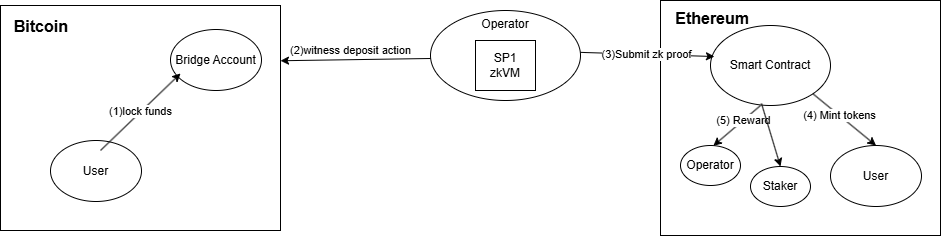
\includegraphics[width=15cm]{img/mint.png}
    \caption{High-level overview of the Minting process in the proposed cross-chain bridge. Users lock BTC on Bitcoin L1, an operator generates a ZK-proof of this lock, and the proof is verified on Ethereum L2 to mint \zktoken\ for the user.}
    \label{fig:mint_overview} % Changed label for specificity
\end{figure}

For \textbf{burning}, a user initiates the process by burning their \zktoken on the Ethereum Layer 2 smart contract. In contrast to traditional bridge designs that might expose a central bridge fund to direct redemption risks, our protocol employs an operator-fronting mechanism. Upon detecting a burn event, an operator fronts the corresponding amount of BTC to the user's designated Bitcoin address. Subsequently, the operator submits a ZK-proof to the Ethereum Layer 2 smart contract, providing cryptographic evidence of the successful Bitcoin transfer to the user. Upon verification of this proof, the operator is reimbursed in \zktoken\ and receives an additional reward for their service. This design mitigates the direct exposure of the primary bridge fund to immediate redemption demands.

\begin{figure}[htb!]
    \centering
    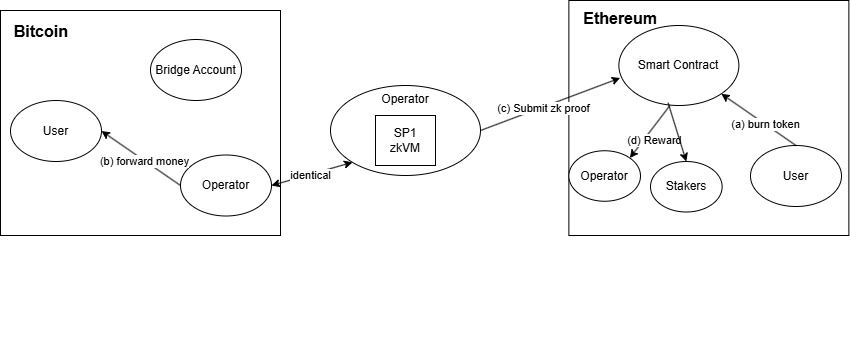
\includegraphics[width=12cm]{img/burn.png}
    \caption{High-level overview of the Burning and Redemption process. Users burn \zktoken\ on Ethereum L2, operators front BTC to the user, and then claim reimbursement and rewards by submitting ZK-proofs of the Bitcoin transfer to the L2 smart contract.}
    \label{fig:burn_overview} 
\end{figure}

The security of the locked Bitcoin funds, critical for maintaining the \zktoken\ peg, is ensured through the implementation of a \textbf{Threshold Signature Scheme (TSS)}. This cryptographic scheme governs the Bitcoin address holding the locked BTC, requiring a predefined threshold of signatures from the TSS participants (stakers) to authorize any transaction. This distributed control significantly minimizes trust in any single entity or small group.


\section{Protocol Design} \label{sec:protocol-design}
Building upon the high-level system architecture presented in Section ~\ref{sec:system_overview}, this section provides a comprehensive and detailed exposition of the proposed cross-chain bridge protocol. It meticulously describes the operational mechanics, cryptographic primitives, and interaction flows that enable trust-minimized asset transfers between Bitcoin Layer 1 and Ethereum Layer 2. Specifically, we delineate the step-by-step processes for asset minting and burning, elaborate on the integration of the zero-knowledge proof system, and detail the application of the Threshold Signature Scheme (TSS) in securing the bridge's locked assets. This section elucidates how the design goals, particularly those related to trust minimization and verifiable execution, are realized at a technical level.
\subsection{Minting Flow} \label{subsec:minting-flow}
Our minting processes starts with a user initiate a Bitcoin transaction. To correctly construct the transaction, user need to first, send to a specific address controlled by the bridge's TSS stakers. Secondly, user need to add a memo output using OP\_RETURN field, it should include the Ethereum Address that will receive the \zktoken. In this way, all important information will be on-chain verifiable, especially the two most important information for the bridge is on-chain; the \textbf{amount} of Bitcoin (BTC) being swapped and the \textbf{reciepient} on Ethereum side receiving the \zktoken. Only if the transaction is correctly constructed, operatrs could then generate a valid ZK-proof, details will be discussed in Section ~\ref{subsec:zk-proof-integration}.

After the deposit is confirmed after 6 confirmations, the operator can generate a ZK-proof attesting to the validity of the deposit transaction. This proof is then submitted to the Ethereum Layer 2 smart contract, which verifies the proof and mints $X-Fee$ of equivalent amount of BTC for \zktoken\ for the user. Noted that the $Fee$ is the operation fee that is for the reward of operators and stakers, details will be discussed in Section ~\ref{sec:economic-model}. 

For each successful ZK-proof submission, the operator receives a reward in \zktoken, which incentivizes them to actively participate in the minting process. This reward mechanism is crucial for maintaining a healthy and competitive operator ecosystem.


\subsection{Burning Flow} \label{subsec:burning-flow}
The burning process is initiated when a user wishes to convert their \zktoken\ back to native BTC. The user executes a burn transaction on the token smart contract deployed on the Ethereum Layer 2 network (e.g., ZkSync Era). This transaction specifies the amount of \zktoken\ to be burned and the target Bitcoin address for redemption. Upon successful execution, the burn request is recorded within the smart contract's state.

Upon recording the burn request, a predefined challenge period commences (e.g., 24 hours). During this period, an operator is incentivized to fulfill the user's redemption request by independently sending the requested amount of native BTC to the specified Bitcoin address from their own funds.

Following the successful BTC transfer to the user, the operator generates a Zero-Knowledge Proof (ZK-proof) attesting to the validity of this delivery transaction on the Bitcoin blockchain. This proof is then submitted to the token smart contract on Ethereum Layer 2. The smart contract meticulously verifies the submitted ZK-proof, cross-referencing the attested Bitcoin transaction details (e.g., recipient address, BTC amount, and transaction finality) against the original burn request recorded earlier. This cryptographic evidence confirms that the operator has successfully executed the specified BTC transfer to the user's designated address.

Upon successful ZK-proof verification, the operator is automatically reimbursed in \zktoken\ from a portion of the burned \zktoken\ and receives a predefined service reward. Stakers also receive a portion of the transaction fees as their reward (detailed economic incentives are discussed in Section ~\ref{sec:economic-model}). This robust incentive structure motivates operators to participate actively in the burning process, thereby ensuring reliable and timely user redemptions of \zktoken\ for native BTC.

A critical safeguard, referred to as the Recovery Mechanism, becomes available if operators fail to deliver the BTC to the user and submit the requisite proof within the stipulated challenge period. In such an event, the user is enabled to manually initiate the reclamation of their burned \zktoken\ back to their wallet. This design choice, which requires explicit user action rather than automatic smart contract execution, is primarily adopted to optimize gas costs associated with frequent on-chain checks and to provide users with direct control over their fund recovery process. This mechanism is crucial for ensuring user fund safety against operator unresponsiveness or malicious inactivity, thereby enhancing the bridge's resilience and user confidence.



\subsection{Smart Contract Architecture} \label{subsec:smart-contract-architecture}
Our cross-chain bridge protocol is structured around two core smart contracts deployed on the Ethereum Layer 2 network (e.g., ZkSync Sepolia Testnet). These contracts collectively manage the intricate logic of the minting and burning processes, ensuring secure and verifiable cross-chain asset transfers.

\begin{enumerate}
	\item \textbf{\texttt{\zktoken} Token Contract:} This contract serves as the primary interface for \texttt{\zktoken} token management, encompassing all core operations related to its lifecycle. It is responsible for maintaining the total supply of \texttt{\zktoken}, managing individual user balances, and facilitating user interaction with their token holdings through minting and burning mechanisms. Furthermore, it incorporates functions for the user-initiated recovery of burned \texttt{\zktoken} in the event of operator unresponsiveness or failure. Beyond core token management, the contract also oversees aspects of the staking system: enabling stakers to claim their accrued rewards, including any accumulated dust from reward distribution, and allowing them to initiate the linear unlocking of their staked funds, subject to predefined minimum unlockable thresholds.
    
    \item \textbf{ZK-Proof Verifier Contract:} This contract \cite{noauthor_sp1-contractscontractssrcisp1verifiergatewaysol_nodate} is exclusively responsible for the cryptographic verification of Zero-Knowledge Proofs. Developed by Succinct Labs, the creators of the SP1 \texttt{zkVM}, this public contract integrates the on-chain verifier necessary for proof validation.
\end{enumerate}

All direct user and external interactions with the bridge's on-chain logic are primarily routed through the \texttt{\zktoken} Token Contract. When an operation necessitates Zero-Knowledge Proof validation, the \texttt{\zktoken} Token Contract initiates an internal call to the ZK-Proof Verifier Contract. Based on the returned verification result, the \texttt{\zktoken} Token Contract then proceeds with the respective subsequent operations, such as minting \texttt{\zktoken} for the user or reimbursing the operator.

\subsection{Zero-Knowledge Proof System Integration} \label{subsec:zk-proof-integration}
Zero-Knowledge Proofs (ZK-proofs) are fundamental to the security and trust-minimization of our cross-chain bridge protocol. They enable the verifiable execution of Bitcoin transaction logic and state transitions on Ethereum Layer 2 without relying on any centralized authorities, federated majorities, oracles, or other trusted intermediaries. This capability is critical for both the minting and burning processes, ensuring that all operations on Ethereum are cryptographically confirmed against the Bitcoin blockchain.

\paragraph{Proof for Minting}
For the minting process, the primary challenge is to cryptographically verify that a user has indeed locked native Bitcoin (BTC) into the bridge's designated Bitcoin address. This is achieved by proving the validity of a Bitcoin transaction that transfers the specified BTC amount to this address. Operators are responsible for constructing and submitting these ZK-proofs. The proof generation process leverages Bitcoin's consensus rules to attest to the following:
\begin{enumerate}
    \item \textbf{Transaction Details Extraction:} From the raw Bitcoin transaction hex, the ZK-proof system extracts critical details, including output addresses, amounts, transaction ID (txid), and the OP\_RETURN memo. It then confirms that one of the output addresses matches the bridge's Bitcoin address and extracts the \texttt{\zktoken} recipient's Ethereum address from the OP\_RETURN memo.
    \item \textbf{Transaction Inclusion Verification:} The proof confirms the transaction's inclusion in a specific Bitcoin block (B\textsubscript{0}). This is achieved by reconstructing the Merkle root of block B\textsubscript{0} from the provided Merkle proof and validating that it matches the Merkle root in the block header of B\textsubscript{0}.
    \item \textbf{Transaction Finality Assurance:} The proof validates the finality of the transaction by verifying a chain of subsequent block headers (B\textsubscript{1} to B\textsubscript{5}). This ensures that each header correctly links to the previous block, confirming 6-block confirmations and thus the high probability of transaction irreversibility, in line with our trust model assumptions regarding Bitcoin network security.
\end{enumerate}
Upon successful generation, the ZK-proof, along with relevant public inputs (e.g., txid, confirmed BTC amount, \texttt{\zktoken} recipient Ethereum address), is submitted to the Ethereum Layer 2 smart contract. The contract then verifies the proof, and if valid, proceeds to mint the corresponding \texttt{\zktoken} for the user.

\paragraph{Proof for Burning}
The burning process also relies on ZK-proofs to ensure trust-minimized operator reimbursement. Here, the operator must cryptographically prove that they have successfully delivered native BTC to the user's specified Bitcoin address in response to a \texttt{\zktoken} burn request. The verification logic for this proof largely mirrors that of the minting process, as both involve proving a Bitcoin transaction that sends some BTC to a designated address. The key distinction lies in the specific target address: for burning, it is the user's Bitcoin address, whereas for minting, it is the bridge's Bitcoin address.

\paragraph{ZK-Proof Composition and On-Chain Verification}
A ZK-proof fundamentally comprises three components: public values, a verification key, and the proof itself.
\begin{itemize}
    \item \textbf{Public Values:} These contain the necessary information that is revealed on-chain and used by the Ethereum smart contract for verification context (e.g., transaction IDs, amounts, recipient addresses).
    \item \textbf{Verification Key:} This represents the specific program or computation that was executed by the prover. Each distinct verification logic (e.g., for minting versus burning) has a unique verification key.
    \item \textbf{Proof:} This is the cryptographic guarantee that the associated program was executed correctly for a specific set of inputs, without revealing the private witness data.
\end{itemize}
Operators submit these ZK-proofs to the Ethereum token smart contract. The smart contract, equipped with the ZK-proof verifier (e.g., utilizing the SP1 zkVM verifier), computationally validates the proof. If the proof is deemed valid, the smart contract executes the corresponding minting or burning operation. This robust mechanism ensures that all cross-chain operations are cryptographically enforced and trust-minimized on Ethereum Layer 2.



\subsection{Threshold Signature Scheme (TSS)} \label{subsec:tss-integration}

The Threshold Signature Scheme (TSS) is the cryptographic primitive underpinning the secure and decentralized custody of the bridge's locked Bitcoin funds. TSS enables the distribution of signing authority among multiple stakers, ensuring that a signature can only be generated if a predefined threshold of stakers cooperates. This mechanism is paramount in a cross-chain bridge context, where the integrity of the entire system hinges on the secure control of the Bitcoin held in escrow.

Specifically, for the Bitcoin address controlling the bridge's locked funds, we implement an $(n, n)$-threshold signature scheme, where $n$ represents the total number of stakers in the protocol's security council. This design choice mandates that \textit{all} stakers must collectively sign a transaction to authorize any withdrawal from the bridge's main vault. Consequently, the security of the locked BTC is preserved as long as at least one staker remains honest and refuses to collude in a malicious transaction. This \textbf{unanimous consent model} provides a stronger safety guarantee than the `t-of-n` honest majority models seen in systems like tBTC v2, as it successfully \textbf{shifts the trust assumption for fund safety from a majority of actors to a single honest staker}.

This stringent $(n, n)$ threshold, while offering maximal security against theft, would be impractical for normal operations. Requiring unanimous consent from all stakers for every user redemption would be highly inefficient and create a severe liveness bottleneck. Our protocol's key innovation is the \textbf{operator-fronting mechanism}, which decouples day-to-day redemption fulfillment from the main vault's security. As detailed in the Section ~\ref{subsec:burning-flow}, operators utilize their own liquid BTC reserves to fulfill user redemption requests. This design cleverly dodges the primary disadvantage of an $(n, n)$ scheme. It allows the bridge to gain the ultimate security benefit of a `1-of-n` trust model for its main capital reserves while maintaining high operational efficiency and liveness through the operator layer.

It is acknowledged, however, that this design makes a deliberate trade-off prioritizing safety. Under extreme conditions where the assumption of operator liquidity fails and the stakers cannot achieve the unanimous consent needed to release funds from the main vault, the redemption process could be stalled. In such a scenario, the bridge would effectively become 'one-way'—minting would continue, and all \texttt{\zktoken} tokens would remain fully backed, but users would be unable to redeem. This outcome represents a conscious design choice, prioritizing the absolute security of the bridge's locked funds over guaranteed liveness in rare, critical failure scenarios.

\section{Trust Model and Foundational Assumptions} \label{sec:trust-model-and-assumption}

This section rigorously defines the trust model of the proposed cross-chain bridge protocol. In the context of a trust-minimized system, it is crucial to explicitly articulate where trust is placed, what assumptions are made about the behavior of participants, and how the protocol's design mitigates risks associated with potential malicious or inactive actors. This analysis underpins the security guarantees and the overall decentralization of the bridge.

The protocol involves three primary actor groups: Users, Operators, and Stakers (Threshold Signature Scheme (TSS) Participants). The adversary model assumes rational, self-interested behavior, wherein actors may deviate from protocol rules if financially incentivized. However, it assumes the presence of at least one honest TSS participant to preserve security.

\subsection{Users}
Users initiate asset transfers, locking BTC for \zktoken\ during minting, and burning \zktoken\ for BTC during redemption.

\paragraph{Trust Assumptions:}
\begin{enumerate}
	\item Users are assumed to be rational and act in their own self-interest, primarily seeking to successfully complete their cross-chain transfers.
	\item Users are responsible for correctly initiating transactions on both Bitcoin L1 (locking BTC) and Ethereum L2 (burning \zktoken).
	\item Users are assumed to possess basic understanding of blockchain interactions (e.g., managing private keys, understanding transaction finality).
\end{enumerate}

\paragraph{Potential Malicious Behavior/Inactivity:}
\begin{enumerate}
\item \textbf{Incorrect Transaction Initiation:} A user may initiate a transaction incorrectly, such as sending BTC to an invalid address or performing a malformed \zktoken\ burn.
\end{enumerate}

\paragraph{Mitigation and Risk Management:}
\begin{enumerate}
\item The protocol design provides clear instructions for user interactions. While the protocol cannot recover funds lost due to user error (e.g., sending to an incorrect address), its on-chain verifiability aims to make outcomes transparent.
\end{enumerate}


\subsection{Operators}
Operators are responsible for observing the Bitcoin L1 chain to detect BTC lock transactions and submitting corresponding zero-knowledge proofs (ZK-proofs) for minting. In the burn process, operators front BTC to users and later reclaim it by submitting ZK-proofs of the \zktoken\ burn event.

\paragraph{Trust Assumptions:}
    \begin{enumerate}
        \item Operators are rational, profit-seeking agents who act honestly when economic incentives (e.g., rewards) exceed operational costs.
        \item Operators possess sufficient BTC liquidity to fulfill redemption requests under normal conditions.
    \end{enumerate}



\paragraph{Potential Malicious Behavior or Inactivity}
    \begin{enumerate}
        \item \textbf{Proof Censorship or Omission (Minting):} An operator may withhold ZK-proofs of valid BTC locks, thereby preventing users from receiving \zktoken.
        \item \textbf{Failure to Front BTC (Burning):} An operator may observe a \zktoken\ burn but refuse to deliver BTC to the user.
        \item \textbf{Proof Censorship or Omission (Reimbursement):} An operator who has fronted BTC might maliciously refuse to submit the proof for reimbursement, potentially to disrupt bridge operations.
        \item \textbf{Submission of Invalid Proofs:} A malicious operator might attempt to submit fraudulent proofs claiming fictitious BTC deposits.
    \end{enumerate}


\paragraph{Mitigations and Trust-Minimization Strategies}
    \begin{enumerate}
        \item \textbf{Open Participation and Redundancy:} The protocol is designed to allow any party, including users themselves, to act as an operator. If one operator fails or censors a proof submission, another operator (or even the user) can submit the required ZK-proof to claim the associated reward, thereby mitigating proof censorship and ensuring operational liveness.
        \item \textbf{Fallback for Non-Delivery (Burning):} A 24-hour recovery mechanism ensures that if no operator delivers BTC and submits proof within the specified window, the user's burned \zktoken\ is returned through reclaim process. This significantly mitigates the risk of user fund loss due to operator inactivity or malicious non-delivery.
        \item \textbf{Economic Disincentive and Protocol Integrity:}Operators have no rational economic incentive to engage in proof censorship or omission during the reimbursement (burn) phase. Failure to submit a valid zk-proof for a legitimate burning request results in the forfeiture of the operator's fronted BTC, as the protocol does not release the locked funds without proof verification. In such a scenario, the user can reclaim the previously burned \zktoken, thereby maintaining a 1:1 peg and preventing any impact on the system's total supply or integrity. The resulting financial loss is borne entirely by the non-cooperative operator, creating a strong disincentive for malicious withholding of proofs.
        \item \textbf{Proof Soundness Guarantees:} The protocol relies on the cryptographic soundness of the SP1 zkVM. Invalid proofs are computationally infeasible to generate and will be rejected by the on-chain verifier, making fraudulent submissions economically irrational for operators who incur proof generation costs.
    \end{enumerate}

\subsection{Stakers / Threshold Signature Scheme (TSS) Participants}
Stakers, who also serve as Threshold Signature Scheme (TSS) participants, collectively control the Bitcoin address holding the bridge's locked BTC. Their primary responsibilities include:
\begin{itemize}
        \item \textbf{Guardianship of Locked Funds:} They are the ultimate custodians of the Bitcoin funds locked within the bridge. This custody is secured through a $(n, n)$-threshold signature scheme, where $n$ out of $n$ participants are required to authorize any transaction from the bridge's Bitcoin address. This setup also applies to the initial funding phase where stakers collectively lock Bitcoin into the bridge.
        \item \textbf{Emergency Redemption Facilitation:} While operators typically use their own liquidity for \texttt{\zktoken} redemptions, stakers are responsible for cooperating to authorize Bitcoin transactions from the bridge's locked funds in emergency scenarios (e.g., if operators universally lack sufficient liquidity). This ensures user redemptions can proceed even under adverse conditions.
        \item \textbf{Protocol Security and Maintenance:} They contribute to the overall security and liveness of the bridge by participating in the TSS protocol, ensuring the integrity of cross-chain operations, and validating the state of the token smart contract.
\end{itemize}

\paragraph{Trust Assumptions:}
    \begin{enumerate}
        \item \textbf{Threshold Honesty for Liveness:} For the bridge to operate reliably and perform legitimate transactions (e.g., emergency redemptions), it is assumed that at least 1 TSS participants are honest and willing to decline malicious transaction proposal by refusing signing.
        \item \textbf{Security Against Unauthorized Spending:} For the prevention of theft or unauthorized spending of locked funds, it is assumed that no more than $n$ TSS participants are malicious and collude. This ensures that a malicious threshold ($n$) cannot be formed to steal funds.
        \item \textbf{Rational Behavior:} TSS participants are assumed to behave rationally, with incentives aligned toward protocol stability due to their substantial staked collateral and reward mechanisms.
        \item \textbf{Cryptographic Security of TSS Components:} The Distributed Key Generation (DKG) process and the FROST signing protocol are cryptographically secure and implemented correctly.
    \end{enumerate}


\paragraph{Potential Malicious Behavior/Inactivity:}
    \begin{enumerate}
        \item \textbf{Collusion Below Threshold (Malign):} A group of fewer than the threshold ($n-1$ or fewer) participants may collude, but they cannot unilaterally control or steal the locked funds due to cryptographic guarantees.

        \item \textbf{Refusal to Sign (Censorship/Liveness Issue):} Stakers might individually or collectively refuse to sign legitimate transactions (e.g., operator reimbursements when operators universally lack BTC liquidity), potentially leading to a stall in redemption operations. This primarily impacts the bridge's liveness rather than its safety (fund security).
    \end{enumerate}

\paragraph{Mitigation and Trust Minimization:}
    \begin{enumerate}
        \item \textbf{Cryptographic Threshold Security:} The core cryptographic properties of FROST (or the chosen TSS scheme) ensure that a threshold of $n$ participants is genuinely required for valid signatures, mathematically preventing unauthorized control by a minority (fewer than $n$ participants).
        \item \textbf{Incentive Alignment for Liveness:} Rational stakers are economically incentivized by rewards to cooperate and fulfill legitimate operations, as failure to do so would impact their own revenue and the protocol's viability. Mechanisms for detecting and penalizing censorship or prolonged inactivity can further enhance liveness.
    \end{enumerate}



\subsection{Underlying Blockchain Trust}
\paragraph{Trust Assumptions:}
\begin{enumerate}
\item \textbf{Bitcoin L1 Security:} It is assumed that Bitcoin Layer 1 operates as intended, without fundamental compromises such as 51\% attacks that could reverse transactions or censorship that could permanently prevent transaction inclusion. Bitcoin's Nakamoto consensus provides sufficient finality (e.g., 6 confirmations for the PoC).
\item \textbf{Ethereum L2 (ZkSync Era) Security:} It is assumed that ZkSync Era functions securely and reliably as a Layer 2 solution, correctly executing smart contracts, processing transactions, and inheriting security from Ethereum L1. This includes the soundness of its rollup mechanism and verifiers.
\end{enumerate}

\paragraph{Potential Malicious Behavior/Inactivity:}
\begin{enumerate}
\item \textbf{51\% Attack on Bitcoin:} A successful 51\% attack could theoretically reverse Bitcoin transactions, affecting locked BTC.
\item \textbf{Critical Bug/Exploit in ZkSync Era:} A major vulnerability in the ZkSync Era protocol could compromise the smart contracts or \zktoken\ tokens.
\end{enumerate}

\paragraph{Mitigation and Risk Management:}
\begin{enumerate}
\item The protocol design relies on the established security properties and decentralization of Bitcoin and Ethereum L2. While these are not directly controlled by the bridge protocol, they form the foundational security layers.
\item The use of 6-block confirmations for Bitcoin transactions is a standard industry practice to ensure a high probability of transaction finality.
\end{enumerate}


\subsection{Adversary Model}
Our analysis considers an adversary who is rational and financially motivated, aiming to maximize profit or disrupt the bridge's operation. Specifically, the adversary is assumed to have:
\begin{itemize}
\item The ability to control a subset of operators, but not necessarily all.
\item The ability to control a minority of TSS participants (fewer than the threshold $n$).
\item Knowledge of the protocol and access to public blockchain data.
\item Access to computational resources, though generating valid ZK-proofs is assumed to be computationally infeasible without the correct witness data.
\end{itemize}
The protocol is designed to maintain its core security properties (fund safety, peg maintenance, eventual liveness) even when facing such an adversary. The primary security goal is to prevent any single point of failure or a minority collusion from compromising the entirety of the locked funds or the bridge's operational integrity.
It is further assumed that the adversary cannot compromise the underlying cryptographic primitives (e.g., zero-knowledge soundness, threshold signature security) nor disrupt the consensus mechanisms of the underlying blockchains.





\section{Economic Model} \label{sec:economic-model}
In this section, we outline the economic incentives and mechanisms that underpin the cross-chain bridge protocol. The economic model is designed to ensure the sustainability and security of the bridge while providing appropriate incentives for users, operators, and stakers (Threshold Signature Scheme (TSS) participants). The model specifically incorporates transaction fees and distinct reward structures for operators and stakers.

\subsection{Value Flows and Reward Distribution}
\label{subsec:value_flow_and_rewward_distribution}
This section details the value flows within the two major operations of the bridge: minting and burning. Each operation involves specific protocol fees and rewards that are distributed among the protocol participants.

\begin{itemize}
    \item \textbf{Minting:} The minting process initiates the flow of value from Bitcoin Layer 1 to Ethereum Layer 2. When a user wishes to mint \texttt{\zktoken}, they lock a specified amount of Bitcoin (\(X\) BTC) on the Bitcoin blockchain. An operator then generates a Zero-Knowledge Proof (ZK-proof) confirming the successful inclusion of this locking transaction on Bitcoin. Upon cryptographic verification of this ZK-proof by the smart contract on Ethereum Layer 2, the corresponding \texttt{\zktoken} is minted and transferred to the user. However, a protocol fee (\(F\)) is deducted from the minted amount. Consequently, the user receives a net amount of \texttt{\zktoken} (\(X'\)) that is less than the initially locked Bitcoin. This relationship can be expressed by the following equation:

\begin{equation} \label{eq:minting_overall}
    X = X' + F_{\text{minting}}
\end{equation}

    Where:
    \begin{itemize}
        \item \(X\): The total amount of BTC locked by the user on the Bitcoin blockchain.
        \item \(X'\): The net amount of \texttt{\zktoken} minted and received by the user on Ethereum Layer 2.
        \item \(F_{\text{minting}}\): The total protocol fee deducted from the minted amount.
    \end{itemize}
    Crucially, despite this fee deduction from the user's received amount, the \texttt{\zktoken} tokens issued (including the portion equivalent to the fee) remain fully backed 1:1 by the total \(X\) BTC locked in the bridge. The fee component (\(F_{\text{minting}}\)) is not removed from backing but rather reallocated to incentivize protocol participants.

    The total protocol fee (\(F_{\text{minting}}\)) is subsequently distributed as rewards to the key participants who facilitate the minting process. This fee is allocated into two primary components: \(R_{\text{operator}}\) for the operator who submitted the ZK-proof, and \(R_{\text{stakers}}\) for the stakers (TSS participants) who secure the bridge's locked funds. Thus, the fee distribution can be further detailed as:

\begin{equation} \label{eq:minting_reward}
    F_{\text{minting}} = R_{\text{operator}} + R_{\text{stakers}}
\end{equation}

    Where:
    \begin{itemize}
        \item \(R_{\text{operator}}\): The reward allocated to the specific operator responsible for generating and submitting the ZK-proof for the minting transaction.
        \item \(R_{\text{stakers}}\): The collective reward designated for all active stakers, which is subsequently divided evenly by the numbers of stakers.
    \end{itemize}
    This economic design ensures that all essential roles in the minting process are appropriately incentivized.

    \item \textbf{Burning:} The burning process facilitates the redemption of \texttt{\zktoken} for native Bitcoin, operating under a distinct economic model that prioritizes the security of the bridge's locked BTC. When a user intends to redeem their \texttt{\zktoken}, they initiate a burn transaction for a specified amount (\(Y\) \texttt{\zktoken}) on the Ethereum Layer 2 smart contract. This action triggers a proof submission window (e.g., 1 day), during which operators are incentivized to fulfill the redemption.

    From the user's perspective, upon a successful burn request, they will receive a net amount of Bitcoin (\(Y'\) BTC) from an operator, after a protocol fee (\(F\)) has been accounted for. The amount of BTC the user receives can be expressed as:

\begin{equation} \label{eq:burning_overall}
    Y = Y' + F_{\text{burning}}
\end{equation}

    Where:
    \begin{itemize}
        \item \(Y\): The total amount of \texttt{\zktoken} burned by the user on Ethereum Layer 2.
        \item \(Y'\): The net amount of BTC received by the user on the Bitcoin blockchain.
        \item \(F_{\text{burning}}\): The total protocol fee associated with the burning operation. This fee is automatically accounted for within the smart contract logic and will be reallocated as detailed below.
    \end{itemize}

    From the operator's perspective, they front the \(Y'\) BTC to the user from their own reserves. To claim reimbursement and rewards, the operator submits a ZK-proof confirming the BTC delivery. The smart contract, upon verifying this proof, reimburses the operator in \texttt{\zktoken} and allocates additional rewards. Specifically, the operator receives \texttt{\zktoken} equivalent to the net amount they fronted (\(Y'\)) plus their operational reward (\(R_{\text{operator}}\)). Stakers, who secure the bridge, receive their collective reward (\(R_{\text{stakers}}\)) from the burned \texttt{\zktoken}. The total fee (\(F_{\text{burning}}\)) is distributed as:

\begin{equation} \label{eq:burning_reward}
    F_{\text{burning}} = R_{\text{operator}} + R_{\text{stakers}}
\end{equation}

    Thus, the total amount of \texttt{\zktoken} that effectively leaves the user's possession (\(Y\)) is reallocated such that the operator receives \(Y'\) \texttt{\zktoken} for reimbursement plus \(R_{\text{operator}}\), and stakers receive \(R_{\text{stakers}}\). The sum of \texttt{\zktoken} transferred to operators and stakers equals the total \texttt{\zktoken} burned by the user (\(Y\)).

    \textbf{Peg Maintenance and Fund Flow:} A crucial aspect of this burning mechanism is its impact on the 1:1 peg between \texttt{\zktoken} and the BTC locked in the bridge's account. Since operators use their own funds to front BTC to users, the Bitcoin held in the bridge's primary reserve remains untouched during standard redemption operations. Simultaneously, the total supply of \texttt{\zktoken} is not reduced through this process; instead, the \texttt{\zktoken} burned by the user is effectively transferred from the user's address to the operators (for reimbursement and reward) and the stakers (for their collective reward). This reallocation of \texttt{\zktoken} ownership, without direct interaction with the locked BTC reserve, ensures that the 1:1 peg between the circulating \texttt{\zktoken} supply and the BTC held in the bridge's secure account is consistently maintained. This design provides robust security by minimizing exposure of the bridge's main liquidity pool.
\end{itemize}


\subsection{Fee Determination and Operator Incentives} \label{subsec:fee_determination}
A crucial aspect of the economic model is the strategic determination of protocol fees to ensure the sustained incentivization of operators. Operators undertake computational and transactional costs, primarily related to generating and submitting Zero-Knowledge Proofs (ZK-proofs) and, in the case of burning, fronting Bitcoin. To ensure operators are consistently incentivized to participate, their expected reward must demonstrably exceed their operational costs. As previously established, the total protocol fee (\(F\)) for both minting and burning operations is allocated equally between the operator and the stakers, meaning the operator's reward (\(R_{\text{operator}}\)) constitutes half of the total protocol fee.

\subsubsection{Minting Fee Condition}
As stated in Equations ~\ref{eq:burning_overall} and ~\ref{eq:burning_reward} (from Section \ref{sec:economic-model}), the minting process involves a protocol fee as reward that is distributed between the operator and stakers. For the operator to be incentivized, the reward they receive must be greater than the gas fee incurred for submitting the ZK-proof to the Ethereum Layer 2 smart contract. This fundamental condition can be expressed as:

\[
R_{\text{operator, mint}} > C_{\text{Ethereum, mint}}
\]

Where:
\begin{itemize}
    \item \(R_{\text{operator, mint}}\): The reward received by the operator for facilitating a minting transaction, denominated in \texttt{\zktoken}.
    \item \(C_{\text{Ethereum, mint}}\): The gas cost incurred by the operator for submitting the minting ZK-proof to the smart contract, denominated in Ether (ETH).
\end{itemize}

Since \(R_{\text{operator, mint}}\) is in \texttt{\zktoken} (which is 1:1 pegged to BTC) and \(C_{\text{Ethereum, mint}}\) is in ETH, a direct comparison requires conversion to a common fiat currency (e.g., USD) to ensure a valid economic assessment. We introduce conversion coefficients:

\begin{itemize}
    \item \(\alpha_{\text{BTC/USD}}\): The conversion ratio from Bitcoin to USD (USD per BTC).
    \item \(\alpha_{\text{ETH/USD}}\): The conversion ratio from Ether to USD (USD per ETH).
\end{itemize}

Applying these conversion factors, the incentivization condition becomes:

\[
\alpha_{\text{BTC/USD}} \cdot R_{\text{operator, mint}} > \alpha_{\text{ETH/USD}} \cdot C_{\text{Ethereum, mint}}
\]

Furthermore, let \(z\) denote the protocol fee rate for minting, expressed as a percentage of the total amount of Bitcoin (\(X\)) the user intends to mint. This means the total protocol fee for minting (\(F_{\text{mint}}\)) can be expressed as \(F_{\text{mint}} = X \cdot z\). As established in Equation 4.2, the operator's reward \(R_{\text{operator, mint}}\) is half of this total protocol fee:

\[
R_{\text{operator, mint}} = \frac{F_{\text{mint}}}{2} = \frac{X \cdot z}{2}
\]

Substituting this into the monetarily converted incentivization condition, we derive the critical relationship for setting the minting fee:

\begin{equation}
\alpha_{\text{BTC/USD}} \cdot \frac{X \cdot z}{2} > \alpha_{\text{ETH/USD}} \cdot C_{\text{Ethereum, mint}}
\end{equation}

This inequality dictates that the protocol fee rate \(z\) must be carefully calibrated such that half of the total fee, when converted to a common value (e.g., USD), sufficiently covers the operator's incurred Ethereum gas costs and provides a positive incentive.

\subsubsection{Burning Fee Condition}
For the burning process, as stated in Equations ~\ref{eq:burning_overall} and ~\ref{eq:burning_reward} (from Section \ref{sec:economic-model}), the protocol fee is also distributed evenly between the operator and stakers. Distinct from minting, the operator incurs two primary costs for a burning transaction:
\begin{enumerate}
    \item The transaction fee for delivering Bitcoin (BTC) to the user on the Bitcoin network (\(C_{\text{Bitcoin}}\)).
    \item The gas fee for submitting the burn ZK-proof to the smart contract on Ethereum Layer 2 (\(C_{\text{Ethereum, burn}}\)).
\end{enumerate}
To ensure operator incentivization, the reward received must be greater than the sum of these two operational costs. This condition can be expressed as:

\[
R_{\text{operator, burn}} > C_{\text{Bitcoin}} + C_{\text{Ethereum, burn}}
\]

Where:
\begin{itemize}
    \item \(R_{\text{operator, burn}}\): The reward received by the operator for facilitating a burning transaction, denominated in \texttt{\zktoken}.
    \item \(C_{\text{Bitcoin}}\): The transaction fee paid by the operator in BTC for sending the redeemed Bitcoin to the user.
    \item \(C_{\text{Ethereum, burn}}\): The gas cost incurred by the operator in Ether (ETH) for submitting the burn ZK-proof to the smart contract.
\end{itemize}

Similar to the minting fee condition, a conversion to a common fiat currency (e.g., USD) is necessary for a valid economic comparison due to the different asset denominations. Utilizing the previously defined conversion coefficients, \(\alpha_{\text{BTC/USD}}\) (for BTC/\zktoken to USD) and \(\alpha_{\text{ETH/USD}}\) (for ETH to USD), the incentivization condition becomes:

\[
\alpha_{\text{BTC/USD}} \cdot R_{\text{operator, burn}} > \alpha_{\text{BTC/USD}} \cdot C_{\text{Bitcoin}} + \alpha_{\text{ETH/USD}} \cdot C_{\text{Ethereum, burn}}
\]

Let \(v\) denote the protocol fee rate for burning, expressed as a percentage of the total amount of \texttt{\zktoken} the user intends to burn (\(Y\)). Thus, the total protocol fee for burning (\(F_{\text{burn}}\)) is \(F_{\text{burn}} = Y \cdot v\). As per Equation ~\ref{eq:burning_overall}, the operator's reward \(R_{\text{operator, burn}}\) is half of this total protocol fee:

\[
R_{\text{operator, burn}} = \frac{F_{\text{burn}}}{2} = \frac{Y \cdot v}{2}
\]

Substituting this into the monetarily converted incentivization condition, we derive the critical relationship for setting the burning fee:

\begin{equation}
\alpha_{\text{BTC/USD}} \cdot \frac{Y \cdot v}{2} > \alpha_{\text{BTC/USD}} \cdot C_{\text{Bitcoin}} + \alpha_{\text{ETH/USD}} \cdot C_{\text{Ethereum, burn}}
\end{equation}

This inequality mandates that the protocol fee rate \(v\) must be appropriately set such that half of the total fee, when converted to a common value, is sufficient to cover both the Bitcoin transaction fees and Ethereum gas costs incurred by the operator, ensuring their sustained participation and profitability.

\subsection{Key Protocol Participants and Incentives}
This section delineates the primary participants within the cross-chain bridge protocol and analyzes their respective economic incentives, costs, and risks, which collectively ensure the system's operational stability and security.

\paragraph{Users:}
Users are individuals or entities seeking to transfer Bitcoin (BTC) value to Ethereum Layer 2 and interact with its decentralized applications.
\begin{itemize}
    \item \textbf{Incentives:} Users are primarily incentivized by the ability to access the broader Ethereum Layer 2 ecosystem, leveraging its higher transaction throughput and lower costs compared to Bitcoin Layer 1, while benefiting from the bridge's trust-minimized architecture.
    \item \textbf{Costs:}
        \begin{itemize}
            \item \textbf{Minting Costs:} Users incur Bitcoin network transaction fees for locking BTC on Layer 1 and Ethereum Layer 2 gas fees for interacting with the smart contract to initiate the minting process. A protocol fee, as detailed in Section ~\ref{subsec:value_flow_and_rewward_distribution}, is also deducted from the minted \texttt{\zktoken}.
            \item \textbf{Burning Costs:} Users pay Ethereum Layer 2 gas fees for interacting with the smart contract to request \texttt{\zktoken} burning. Additionally, a protocol fee is deducted from the redeemed BTC amount, as outlined in Section ~\ref{subsec:value_flow_and_rewward_distribution}. A contingent cost may arise for initiating the recovery mechanism if an operator fails to deliver BTC within the designated challenge period.
        \end{itemize}
\end{itemize}   
    
\paragraph{Operators:}
Operators are entities responsible for monitoring on-chain transactions, generating and submitting Zero-Knowledge Proofs (ZK-proofs) to the smart contract, and fronting liquidity for \texttt{\zktoken} redemptions.
\begin{itemize}
    \item \textbf{Incentives:} Operators are primarily incentivized through rewards (specifically \(R_{\text{operator}}\allowbreak\), as defined in Section ~\ref{subsec:value_flow_and_rewward_distribution}) for successfully submitting valid ZK-proofs that confirm Bitcoin lock-ins for minting or Bitcoin deliveries for burning. These rewards are paid in \texttt{\zktoken}.
    \item \textbf{Costs and Risks:}
        \begin{itemize}
            \item \textbf{Operational Costs:} Operators incur Ethereum Layer 2 gas fees for submitting ZK-proofs to the smart contract during both minting and burning processes.
            \item \textbf{Liquidity Risk (Burning):} During burning, operators must front BTC to users from their own liquidity. There is a risk that an operator who fronts BTC might not be the one to successfully submit the corresponding ZK-proof within the challenge window. In such a scenario, the operator who successfully submits the ZK-proof will receive the reimbursement and reward, potentially leaving the initial fronting operator un-reimbursed for their capital.
        \end{itemize}
\end{itemize}    
    

\paragraph{Stakers}
Stakers are individuals or entities who secure the bridge's locked Bitcoin funds by staking their own collateral and participating in the Threshold Signature Scheme (TSS), including contributing to the initial funding of the bridge.
\begin{itemize}
    \item \textbf{Incentives:} Stakers receive a portion of the protocol's transaction fees (specifically \(R_{\text{stakers}}\), as defined in Section ~\ref{subsec:value_flow_and_rewward_distribution}) for each successful minting and burning operation. This incentivizes their active participation in maintaining the bridge's security and integrity. Their staked collateral also aligns their economic interests with the bridge's stability, as malicious actions would result in significant financial loss.
    \item \textbf{Risks and Disincentives:} Stakers face the risk of losing their staked collateral through all stakers collusion.
\end{itemize}

    


\chapter{Implementation} \label{chap:implementation}
\thispagestyle{empty}
This section details the practical realization of the proposed trust-minimized cross-chain bridge protocol. It describes how the design principles outlined in Section~\ref{sec:protocol-design}, particularly the Minting Flow (Section~\ref{subsec:minting-flow}), Burning Flow (Section~\ref{subsec:burning-flow}), Smart Contract Architecture (Section~\ref{subsec:smart-contract-architecture}), Zero-Knowledge Proof System Integration (Section~\ref{subsec:zk-proof-integration}), and Threshold Signature Scheme (TSS) (Section~\ref{subsec:tss-integration}), were translated into a functional system.

\section{Smart Contract Implementation}
This section details the realization of the bridge's on-chain logic, which is primarily managed through a set of smart contracts deployed on Ethereum Layer 2 (e.g., ZkSync Era Testnet). The \textbf{\texttt{\zktoken} Token Contract} serves as the core protocol contract, responsible for managing the bridge's state, \texttt{\zktoken} issuance, staker interactions, and coordinating cryptographic proof verifications. A separate ZK-proof verifier contract, developed by Succinct Labs, is utilized as a public, audited component for validating Zero-Knowledge Proofs. This verifier contract is called internally by the \texttt{\zktoken} token contract, allowing us to focus our implementation details on the core bridge logic within the \texttt{\zktoken} token contract itself.

\subsection{zkBTC Token Contract Setup}
The \texttt{\zktoken} token contract is implemented in Solidity. Conceptually, for a fully trust-minimized deployment, the token contract is designed to be managed and deployed by the stakers through a Threshold Signature Scheme (TSS) signing mechanism, where stakers are required to unanimously sign and deploy the contract with appropriate initial parameters.

For the Proof-of-Concept (PoC), a simplified and less decentralized smart contract setup has been implemented. In this PoC, the smart contract is deployed directly by the developers rather than the stakers, which is sufficient for the purpose of testing the protocol's core functionalities. The methodology for a fully trust-minimized setup utilizing TSS will be discussed further in Section ~\ref{subsec:trust_minimized_kickstart}.

\subsubsection{Key Contract Constants}
Critical parameters governing the economic model and operational thresholds are defined as immutable constants within the \texttt{\zktoken} token contract to ensure predictable and secure behavior. These constants are initialized during deployment and cannot be altered thereafter. Table~\ref{tab:contract_constants} lists the key constants with their values and descriptions.

\begin{table}[htbp]
\label{tab:contract_constants}
\centering
\small
\begin{tabularx}{\textwidth}{|X|X|X|} % X will fill the remaining width
\hline
\textbf{Constant Name} & \textbf{Value} & \textbf{Description} \\
\hline
\texttt{FEE} & \texttt{20} & Protocol fee applied to both minting and burning operations, expressed in basis points (100 basis points = 1\%). This fee is 0.2\%. \\
\hline
\texttt{SATOSHI\allowbreak\_TO\allowbreak\_\zktoken} & \texttt{10\textasciicircum{}10} & Conversion factor defining the relationship between Bitcoin satoshis and \texttt{\zktoken} units. Since \texttt{\zktoken} uses 18 decimal places (like Ethereum), 1 satoshi (10\textasciicircum{}8 BTC) corresponds to 10\textasciicircum{}10 \texttt{\zktoken} units. \\
\hline
\texttt{INITIAL\allowbreak\_MINT\allowbreak\_PER\allowbreak\_STAKER} & \texttt{1 * 1e18} & Represents the initial amount of \texttt{\zktoken} allocated per staker during the bridge's bootstrap phase (e.g., 1 \texttt{\zktoken} with 18 decimals). \\
\hline
\texttt{FOREVER\allowbreak\_LOCKED\allowbreak\_PER\allowbreak\_STAKER} & \texttt{INITIAL\allowbreak\_MINT\allowbreak\_PER\allowbreak\_STAKER\allowbreak{} / 10} & The proportion of \texttt{\zktoken} that remains permanently locked per staker, intended to align long-term incentives (e.g., 10\% of initial mint). \\
\hline
\texttt{INITIAL\allowbreak\_UNLOCK\allowbreak\_DURATION} & \texttt{360 days} & The duration over which a staker's initially locked \texttt{\zktoken} gradually becomes available for unlocking. \\
\hline
\texttt{SUBMISSION\allowbreak\_PERIOD} & \texttt{1 days} & The fixed time window for operators to submit a ZK-proof for a burning transaction, after which a user can initiate an auto-recovery. \\
\hline
\texttt{MIN\allowbreak\_MINTING\allowbreak\_AMOUNT} & \texttt{1*\allowbreak{}SATOSHI\allowbreak\_TO\allowbreak\_\zktoken} & The minimum amount of Bitcoin (in satoshis) that a user can mint into \texttt{\zktoken} (e.g., equivalent to 1 satoshi). \\
\hline
\end{tabularx}
\caption{Key Constants in the \texttt{\zktoken} Token Contract}
\end{table}

These constants play a critical role in defining the economic parameters, security thresholds, and operational timelines of the bridge, ensuring predictable behavior and participant incentives. For instance, \texttt{FEE}, directly influences the value flows described in the Economic Model (Section ~\ref{sec:economic-model}).

\subsubsection{Constructor Parameters}
Following the declaration of constants, the contract's constructor is responsible for initializing its mutable state variables upon deployment. This sets up its initial operational environment. For the Proof-of-Concept, the constructor is designed to take five essential parameters, configuring the core components and initial participants of the bridge.

The parameters passed during deployment are:
\begin{enumerate}
    \item \textbf{\texttt{\_verifier} (address):} This is the Ethereum address of the ZK-proof verifier contract. As noted earlier, this is an open-source contract developed by Succinct Labs, typically deployed to various networks with publicly available addresses. For standard deployments, it's generally utilized as a pre-deployed public contract.
    \item \textbf{\texttt{\_programVKey\_mint} (bytes32):} This represents the unique verification key for the Bitcoin minting ZK-proof circuit. It cryptographically defines the specific ZK program that validates Bitcoin lock-in transactions.
    \item \textbf{\texttt{\_programVKey\_burn} (bytes32):} Similarly, this is the verification key for the Bitcoin burning ZK-proof circuit. It defines the ZK program responsible for validating Bitcoin delivery transactions by operators.
    \item \textbf{\texttt{\_bridge\_address} (string memory):} This parameter specifies the Bitcoin address controlled by the bridge's stakers (Threshold Signature Scheme (TSS) participants), indicating where the BTC funds are locked.
    \item \textbf{\texttt{\_stakers} (address[] memory):} This is an array containing the Ethereum addresses of the initial set of stakers. These stakers are assumed to have pre-deposited a specific amount of BTC into the bridge's Bitcoin address offline.
\end{enumerate}

During the constructor's execution, the contract performs critical initializations. It sets up the core functionalities by assigning the provided verifier and program verification keys to internal state variables. Crucially, it iterates through the list of initial stakers. For each staker, the contract checks for validity (e.g., non-zero address, not already registered) and then performs an initial minting of \texttt{\zktoken} for them. This initial minting is based on the \texttt{INITIAL\_MINT\_PER\_STAKER} constant and allocates amounts for \texttt{stakerInitialLocked} and \texttt{stakerForeverLocked}, along with setting their initial unlock times.


The Solidity code for the constructor is provided below:

\begin{lstlisting}[language=Solidity, caption=\zktoken Token Contract Constructor, label=lst:constructor]
constructor(
    address _verifier,
    bytes32 _programVKey_mint,
    bytes32 _programVKey_burn,
    string memory _bridge_address,
    address[] memory _stakers
) ERC20("Zero-Knowledge Bitcoin", "\zktoken") Ownable(msg.sender) {
    verifier = _verifier;
    programVKey_mint = _programVKey_mint;
    programVKey_burn = _programVKey_burn;
    BRIDGE_ADDRESS = _bridge_address;

    require(_stakers.length > 0, "Stakers required");
    for (uint256 i = 0; i < _stakers.length; i++) {
        address s = _stakers[i];
        require(s != address(0) && !isStaker[s], InitializationStakerListError());
        stakers.push(s);
        isStaker[s] = true;
        // Initial mint logic:
        _mint(s, INITIAL_MINT_PER_STAKER);
        stakerInitialLocked[s] = INITIAL_MINT_PER_STAKER;
        stakerUnlocked[s] = 0;
        stakerLastUnlockTime[s] = block.timestamp;
        stakerForeverLocked[s] = FOREVER_LOCKED_PER_STAKER;
    }
    initialMinted = true;
    initialMintUnlockStart = block.timestamp;
    initialMintUnlockEnd = block.timestamp + INITIAL_UNLOCK_DURATION;
}
\end{lstlisting}


\subsection{Minting Logic}
The minting process is initiated when a user successfully deposits Bitcoin into the bridge's designated address on Bitcoin Layer 1, and an operator generates a valid Zero-Knowledge Proof (ZKP) confirming this deposit. The operator then submits this proof to the \texttt{\zktoken} token contract on Ethereum Layer 2. The contract's primary function for this operation is \texttt{verifyAndMint}, which performs a series of verifications and calculations before issuing new \texttt{\zktoken} tokens.

The \texttt{verifyAndMint} function first validates the submitted ZK-proof using the integrated ZK-proof verifier contract. Upon successful proof verification, the function proceeds to decode the public inputs from the proof, extracting critical information such as the Bitcoin transaction ID, the recipient's Ethereum address, and the deposited Bitcoin amount. Rigorous checks are then performed to ensure the legitimacy of the mint request, including verifying that the transaction ID has not been previously processed, the proof itself is valid (as indicated by a flag in public inputs), the minting amount is positive, and the recipient address is valid.

Once all preliminary checks pass, the contract converts the deposited Bitcoin amount (which typically has 8 decimal places) to the \texttt{\zktoken} token's 18 decimal places using a predefined conversion factor. It then verifies that the converted amount meets a minimum minting threshold. A protocol fee is subsequently deducted from the total converted amount to cover operational costs and incentivize network participants. The remaining net amount is minted to the user's specified Ethereum address. The deducted fee is then split, with a portion minted directly to the calling operator as a reward for their service, and the remaining portion allocated as a reward for all active stakers. For gas efficiency, staker rewards are not distributed individually in real-time but are instead accumulated within the contract for later claim or distribution, the specifics of which are detailed in Section~\ref{subsec:staker-related-logic}.

The algorithmic flow for the \texttt{verifyAndMint} function is detailed in Algorithm~\ref{alg:minting_logic}.


\begin{algorithm}
\caption{Minting Logic (\texttt{verifyAndMint} function)}
\label{alg:minting_logic}
\begin{algorithmic}[1] % Using [1] for line numbering
    \Procedure{verifyAndMint}{\_publicValues, \_proofBytes}
        \State \textbf{Input:} \texttt{\_publicValues} (bytes), \texttt{\_proofBytes} (bytes)
        \State \textbf{Output:}\allowbreak\ \texttt{tx\_id} (bytes32), \texttt{depositer\_address} (address), \texttt{userAmount} (uint256), \texttt{is\_valid} (bool)
        \State
        \State // --- Proof Verification ---
        \If{NOT \texttt{ISP1Verifier(verifier).verifyProof(programVKey\allowbreak\_mint, \allowbreak\_publicValues, \allowbreak\_proofBytes)}}
            \State \textbf{Revert} "Invalid proof from verifier"
        \EndIf
        \State
        \State // --- Decode Public Inputs ---
        \State (\texttt{tx\_id}, \texttt{depositer\_address}, \texttt{amount}, \texttt{is\_valid}) $\gets$ \texttt{abi.decode(\_publicValues)}
        \State
        \State // --- Pre-Minting Validations ---
        \State \textbf{Require} \texttt{tx\_id} NOT in \texttt{processedTxIds} (MintingRequestAlreadyProcessed)
        \State \textbf{Require} \texttt{is\_valid} IS \texttt{true} (InvalidProof)
        \State \textbf{Require} \texttt{amount} $> 0$ (MintingAmountZero)
        \State \textbf{Require} \texttt{depositer\_address} IS NOT zero address (InvalidAddress)
        \State
        \State // --- Mark Transaction Processed ---
        \State \texttt{processedTxIds[tx\_id]} $\gets$ \texttt{true}
        \State
        \State // --- Amount Conversion and Validation ---
        \State \texttt{amount} $\gets$ \texttt{amount} $\times$ \texttt{SATOSHI\_TO\_\zktoken} (Convert to 18 decimals)
        \State \textbf{Require} \texttt{amount} $\ge$ \texttt{MIN\_MINTING\_AMOUNT} (MintingAmountTooSmall)
        \State
        \State // --- Fee Calculation and Distribution ---
        \State \texttt{userAmount} $\gets$ \texttt{amount} $\times$ (10000 - \texttt{FEE}) / 10000
        \State \texttt{feeAmount} $\gets$ \texttt{amount} - \texttt{userAmount}
        \State \texttt{operatorReward} $\gets$ \texttt{feeAmount} / 2
        \State \texttt{stakerReward} $\gets$ \texttt{feeAmount} - \texttt{operatorReward}
        \State
        \State // --- Token Minting ---
        \State \texttt{\_mint(depositer\_address, userAmount)}
        \State \texttt{\_mint(msg.sender, operatorReward)}
        \State \texttt{\_mint(address(this), stakerReward)} // Mint to contract for staker pool
        \State \texttt{\_addRewardToStakers(stakerReward)} // Update internal staker reward balance
        \State
        \State // --- Emit Events ---
        \State \textbf{Emit} \texttt{OperatorReward(msg.sender, operatorReward)}
        \State \textbf{Emit} \texttt{ProofVerifiedAndMinted(tx\_id, depositer\_address, userAmount, is\_valid)}
        \State
        \State \textbf{Return} (\texttt{tx\_id}, \texttt{depositer\_address}, \texttt{userAmount}, \texttt{is\_valid})
    \EndProcedure
\end{algorithmic}
\end{algorithm}

\subsection{Burning Logic} \label{subsec:burning-logic}
The burning process facilitates the redemption of \texttt{\zktoken} on Ethereum Layer 2 for native Bitcoin on Layer 1. This process is structured into two main operational flows: the user initiating a burn request and an operator subsequently submitting a Zero-Knowledge Proof (ZKP) to confirm the Bitcoin transfer. These flows correspond to two distinct functions within the smart contract: \texttt{initiateBurn} and \texttt{submitBurnProof}.

\subsubsection{\texttt{initiateBurn}}
The \texttt{initiateBurn} function allows a user to request the burning of their \texttt{\zktoken} tokens in exchange for Bitcoin. The user calls this function, providing two key parameters: the amount of \texttt{\zktoken} they wish to burn and their Bitcoin address for receiving the redeemed BTC.

Upon invocation, the function first performs essential validation checks: it verifies that the user's \texttt{\zktoken} balance is sufficient for the requested amount and that the requested amount meets a predefined minimum burning threshold. Following successful validation, the contract proceeds to calculate the actual amount of \texttt{\zktoken} to be burned after deducting a protocol fee. This net amount is then converted to its equivalent value in Bitcoin satoshis. A notable aspect of this conversion is the handling of "dust" amounts: since ERC-20 tokens typically utilize 18 decimal places while Bitcoin operates with 8, there may be a small remainder of \texttt{\zktoken} that cannot be precisely represented as whole satoshis. This dust amount is accounted for and is designed to be returned to the user later when the burn request is fulfilled.

Crucially, upon successful initiation, the specified amount of \texttt{\zktoken} from the user's balance is \textbf{transferred temporarily to the token smart contract itself}, rather than being immediately destroyed (i.e., reducing the total supply). These tokens are held in escrow within the contract until the burn request is either successfully fulfilled by an operator or reclaimed by the user in case of operator failure, ensuring that the tokens remain backed by Bitcoin until the final resolution.

Finally, the function records all pertinent details of the burn request, including the user's address, the amounts involved (gross, net, dust), the target Bitcoin address, and a timestamp. This stored information becomes queryable by operators, enabling them to identify and fulfill pending burn requests. The algorithmic steps of the \texttt{initiateBurn} function are summarized in Algorithm~\ref{alg:initiate_burn}.

\begin{algorithm}
\caption{Initiate Burn Logic (\texttt{initiateBurn} function)}
\label{alg:initiate_burn}
\begin{algorithmic}[1]
	\Procedure{initiateBurn}{amountRequestBurn\zktoken, btcAddress}
		\State \textbf{Input:} \texttt{amountRequestBurn\zktoken} (uint256), \texttt{btcAddress} (string)
		\State \textbf{Effect:} Records a burn request, transfers \texttt{\zktoken} from user to contract
        \State
        \State // --- Pre-Conditions ---
        \State \textbf{Require} \texttt{balanceOf(msg.sender)} $\ge$ \texttt{amountRequestBurn\zktoken} (BurnInsufficientBalance)
        \State \textbf{Require} \texttt{amountRequestBurn\zktoken} $\ge$ \texttt{MIN\_BURNING\_AMOUNT} (BurnAmountTooSmall)
        \State
        \State // --- Fee Calculation ---
        \State \texttt{feeAmount} $\gets$ (\texttt{amountRequestBurn\zktoken} $\times$ \texttt{FEE}) / 10000
        \State \texttt{zkBTCAvailable} $\gets$ \texttt{amountRequestBurnzkBTC} - \texttt{feeAmount}
        \State
        \State // --- Convert to Satoshi \& Calculate Dust ---
        \State \texttt{userSatoshi} $\gets$ \texttt{zkBTCAvailable} / \texttt{SATOSHI\_TO\_zkBTC}
        \State \texttt{actualzkBTCSent} $\gets$ \texttt{userSatoshi} $\times$ \texttt{SATOSHI\_TO\_\zktoken}
        \State \texttt{dust} $\gets$ \texttt{zkBTCAvailable} - \texttt{actualzkBTCSent}
        \State
        \State // --- Allocate Rewards from Fee ---
        \State \texttt{operatorReward} $\gets$ \texttt{feeAmount} / 2
        \State \texttt{stakerReward} $\gets$ \texttt{feeAmount} - \texttt{operatorReward}
        \State
        \State // --- Transfer \zktoken to Contract ---
        \State \texttt{\_transfer(msg.sender, address(this),\allowbreak amountRequestBurnzkBTC)}
        \State
        \State // --- Store Burn Request ---
        \State \texttt{burnRequests[nextBurnId]} $\gets$ new \texttt{BurnRequest} {
            \State \quad \texttt{user: msg.sender},
            \State \quad \texttt{total\_amount: amountRequestBurnzkBTC},
            \State \quad \texttt{zkBTCToReimburse: actualzkBTCSent},
            \State \quad \texttt{exactBtcUserReceive: userSatoshi},
            \State \quad \texttt{rewardOperator: operatorReward},
            \State \quad \texttt{rewardStaker: stakerReward},
            \State \quad \texttt{dust: dust},
            \State \quad \texttt{btcAddress: btcAddress},
            \State \quad \texttt{timestamp: block.timestamp},
            \State \quad \texttt{fulfilled: false},
            \State \quad \texttt{reclaimed: false}
        }
        \State
        \State // --- Emit Event \& Increment ID ---
        \State \textbf{Emit} \texttt{BurnInitiated(nextBurnId, msg.sender, userSatoshi, btcAddress)}
        \State \texttt{nextBurnId} $\gets$ \texttt{nextBurnId} + 1
    \EndProcedure
\end{algorithmic}
\end{algorithm}


\subsubsection{\texttt{submitBurnProof}}
The \texttt{submitBurnProof} function is invoked by an operator subsequent to successfully transferring the corresponding Bitcoin (BTC) to the user's specified address on Bitcoin Layer 1. This function requires three primary parameters from the operator: a unique \texttt{burnId} to identify the fulfilled burn request, and the Zero-Knowledge Proof (ZKP) components, namely \texttt{\_publicValues} and \texttt{\_proofBytes}.

Upon receiving these parameters, the function first performs critical preliminary checks: it verifies the existence of the burn request corresponding to the provided \texttt{burnId}, ensures that the request has not been previously fulfilled, and confirms that the submission occurs within the designated validity period (i.e., the request has not expired). Following these initial validations, the contract proceeds to verify the cryptographic validity of the submitted ZKP by interacting with the designated ZK-proof verifier contract.

If the ZKP is successfully validated, the public inputs (\texttt{\_publicValues}) are decoded to extract essential information: the user's Bitcoin recipient address, the exact amount of BTC transferred in satoshis, and a boolean flag indicating the proof's validity. Further crucial checks are then executed: the contract verifies that the Bitcoin address specified in the proof matches the recipient address recorded in the original burn request, and that the amount of BTC confirmed in the proof is equal to or greater than the amount the user was expected to receive.

Once all verifications are passed, the burn request is irrevocably marked as fulfilled within the contract's state. Subsequently, the \texttt{\zktoken} tokens temporarily held in escrow by the smart contract (transferred during `initiateBurn`) are precisely distributed: a portion is transferred to the operator as reimbursement for the fronted BTC and as a reward for their service, another portion is allocated to the staker reward pool, and any residual "dust" amount (too small to be represented as whole satoshis) is returned to the original user's Ethereum address. The final algorithmic steps involve updating the staker reward balance and emitting relevant events to signal the successful fulfillment of the burn request. The detailed algorithmic flow for \texttt{submitBurnProof} is presented in Algorithm~\ref{alg:submit_burn_proof}.

\begin{algorithm}
\caption{Submit Burn Proof Logic (\texttt{submitBurnProof} function)}
\label{alg:submit_burn_proof}
\begin{algorithmic}[1]
    \Procedure{submitBurnProof}{burnId, \_publicValues, \_proofBytes}
        \State \textbf{Input:} \texttt{burnId} (uint256), \texttt{\_publicValues} (bytes), \texttt{\_proofBytes} (bytes)
        \State \textbf{Effect:} Finalizes a burn request, distributes \texttt{\zktoken}, updates state
        \State
        \State // --- Retrieve and Validate Burn Request ---
        \State \texttt{request} $\gets$ \texttt{burnRequests[burnId]}
        \State \textbf{Require} \texttt{request.user} IS NOT zero address (BurnRequestNotFound)
        \State \textbf{Require} \texttt{request.fulfilled} IS \texttt{false} (BurnAlreadyFulfilled)
        \State \textbf{Require} \texttt{block.timestamp} $\le$ \texttt{request.timestamp} + \texttt{SUBMISSION\_PERIOD} (BurnRequestExpired)
        \State
        \State // --- ZK-Proof Verification ---
        \If{NOT \texttt{ISP1Verifier(verifier).verifyProof(programVKey\_burn, \_publicValues, \_proofBytes)}}
            \State \textbf{Revert} "Invalid proof"
        \EndIf
        \State
        \State // --- Decode Public Inputs from Proof ---
        \State (\texttt{user\_btc\_address}, \texttt{amount}, \texttt{is\_valid}) $\gets$ \texttt{abi.decode(\_publicValues)}
        \State
        \State // --- Post-Proof Validations ---
        \State \textbf{Require} \texttt{is\_valid} IS \texttt{true} (InvalidProof)
        \State \textbf{Require} \texttt{keccak256(request.btcAddress)} == \texttt{keccak256(user\_btc\_address)} (OperatorSendWrongRecipent)
        \State \textbf{Require} \texttt{amount} $\ge$ \texttt{request.exactBtcUserReceive} (OperatorUnderpaid)
        \State
        \State // --- Mark Request Fulfilled ---
        \State \texttt{request.fulfilled} $\gets$ \texttt{true}
        \State
        \State // --- Distribute Escrowed \zktoken ---
        \State \texttt{\_transfer(address(this),\allowbreak msg.sender,\allowbreak request.\zktoken ToReimburse \allowbreak)}
        \State \texttt{\_transfer(address(this), msg.sender,\allowbreak request.rewardOperator)}
        \State \texttt{\_transfer(address(this), request.user, request.dust)}
        \State
        \State // --- Update Staker Rewards ---
        \State \texttt{\_addRewardToStakers(request.rewardStaker)}
        \State
        \State // --- Emit Events ---
        \State \textbf{Emit} \texttt{OperatorReward(msg.sender, request.rewardOperator)}
        \State \textbf{Emit} \texttt{BurnFulfilled(burnId, msg.sender)}
    \EndProcedure
\end{algorithmic}
\end{algorithm}


\subsection{Staker-Related Logic} \label{subsec:staker-related-logic}
This section elucidates the mechanisms governing staker participation, focusing on two critical aspects: an efficient method for stakers to collect accumulated rewards and the gradual release of their locked collateral. The design prioritizes gas efficiency for reward distribution, given the potentially large number of stakers in a trust-minimized bridge environment.

\subsubsection{Reward Distribution Mechanism}
The bridge's design fosters broad participation by allowing any entity to become a staker upon depositing sufficient collateral. This open participation model necessitates a highly gas-efficient reward distribution system. Traditional direct token transfers to each staker upon every reward trigger (e.g., after each minting or burning event) would incur prohibitive gas costs, particularly as the number of stakers grows. Such an approach would disproportionately burden operators, potentially disincentivizing their participation or leading to increased operational fees.

To circumvent these inefficiencies, the protocol employs a "pull" mechanism for reward collection. Instead of pushing rewards to individual stakers, the contract maintains a cumulative record of rewards and tracks each staker's collected amount. This allows stakers to claim their accumulated rewards on demand, thereby externalizing the gas costs of individual claims to the staker themselves. The uncollected reward for a given staker can then be determined by the difference between the total accumulated reward per staker and the amount they have previously claimed.

\paragraph{Internal Reward Accumulation (\texttt{\_addRewardToStakers})}
The internal function \texttt{\_addRewardToStakers} is responsible for atomically calculating and accumulating staker rewards. It is invoked whenever a new reward pool is generated from bridge fees (e.g., during successful mint or burn operations). The function first validates that the `totalReward` is positive and that there is at least one active staker. The total reward is then divided equally among all active stakers, with any remainder being accounted for as "dust" to preserve precision.

Let $R_T$ denote the `totalReward` and $N$ denote `stakers.length`. The `rewardPerStaker` ($R_{PS}$) and `dust` ($D$) from a given reward distribution are calculated as:
\[
R_{PS} = \lfloor R_T / N \rfloor
\]
\[
D = R_T - (R_{PS} \times N)
\]
The calculated `rewardPerStaker` is then added to a global `cumulativeRewardPerStaker` variable, and the `dust` is added to a separate `dustCollected` variable. This ensures that all reward value is tracked. The algorithmic flow is presented in Algorithm~\ref{alg:add_reward_to_stakers}.

\begin{algorithm}[htbp]
\caption{Internal Reward Accumulation (\texttt{\_addRewardToStakers})}
\label{alg:add_reward_to_stakers}
\begin{algorithmic}[1]
    \Procedure{\_addRewardToStakers}{totalReward}
        \State \textbf{Input:} \texttt{totalReward} (uint256)
        \State \textbf{Effect:} Updates global cumulative staker reward balances
        \State
        \State // --- Pre-Conditions ---
        \State \textbf{Require} \texttt{stakers.length} $> 0$ (StakerRequired)
        \State \textbf{Require} \texttt{totalReward} $> 0$ (RewardZero)
        \State
        \State // --- Calculate Per-Staker Reward and Dust ---
        \State \texttt{n} $\gets$ \texttt{stakers.length}
        \State \texttt{rewardPerStaker} $\gets$ \texttt{totalReward} / \texttt{n}
        \State \texttt{dust} $\gets$ \texttt{totalReward} - (\texttt{rewardPerStaker} $\times$ \texttt{n})
        \State
        \State // --- Update Global Accumulators ---
        \State \texttt{cumulativeRewardPerStaker} $\gets$ \texttt{cumulativeRewardPerStaker} + \texttt{rewardPerStaker}
        \State \texttt{dustCollected} $\gets$ \texttt{dustCollected} + \texttt{dust}
        \State
        \State // --- Emit Events ---
        \State \textbf{Emit} \texttt{StakerRewardAdded(totalReward)}
        \State \textbf{Emit} \texttt{StakerDustAdded(dust)}
    \EndProcedure
\end{algorithmic}
\end{algorithm}

\paragraph{User-Initiated Reward Collection (\texttt{claimStakerReward})}
The \texttt{claimStakerReward} function enables individual stakers to retrieve their accumulated rewards. A caller must first be verified as an active staker. The function then calculates the unclaimed reward amount by subtracting the staker's previously `claimedReward` from the current `cumulativeRewardPerStaker`. If a positive unclaimed amount is found, the staker's `claimedReward` record is updated to the current `cumulativeRewardPerStaker` value, and the calculated reward is transferred from the contract's balance to the staker. The algorithmic steps are detailed in Algorithm~\ref{alg:claim_staker_reward}.

\begin{algorithm}[htbp]
\caption{User-Initiated Reward Collection (\texttt{claimStakerReward})}
\label{alg:claim_staker_reward}
\begin{algorithmic}[1]
    \Procedure{claimStakerReward}{}
        \State \textbf{Effect:} Transfers accumulated reward to the calling staker
        \State
        \State // --- Pre-Conditions ---
        \State \textbf{Require} \texttt{isStaker[msg.sender]} IS \texttt{true} (NotStaker)
        \State
        \State // --- Calculate Unclaimed Reward ---
        \State \texttt{reward} $\gets$ \texttt{cumulativeRewardPerStaker} - \texttt{claimedReward[msg.sender]}
        \State \textbf{Require} \texttt{reward} $> 0$ (NoRewardToClaim)
        \State
        \State // --- Update Claimed Amount and Transfer Reward ---
        \State \texttt{claimedReward[msg.sender]} $\gets$ \texttt{cumulativeRewardPerStaker}
        \State \texttt{\_transfer(address(this), msg.sender, reward)}
        \State
        \State // --- Emit Event ---
        \State \textbf{Emit} \texttt{StakerRewardClaimed(msg.sender, reward)}
    \EndProcedure
\end{algorithmic}
\end{algorithm}

\paragraph{Dust Management (\texttt{distributeDust})}
The \texttt{distributeDust} function addresses the fractional \texttt{\zktoken} amounts (dust) that accumulate from the division operations in `\_addRewardToStakers`. This function allows for the distribution of accumulated dust when a sufficient amount has gathered to provide at least 1 \texttt{\zktoken} (in its 18 decimal representation) per staker. It first checks if the total `dustCollected` is at least equal to the number of active stakers. If so, a `dustPerStaker` amount is calculated and added to the `cumulativeRewardPerStaker`, making it claimable through `claimStakerReward`. The remainder (new dust) is retained in `dustCollected`. This function is expected to be called infrequently, primarily when the collected dust becomes significant enough to warrant the gas cost of its distribution, thereby maintaining the protocol's precision. The algorithmic flow is presented in Algorithm~\ref{alg:distribute_dust}.

\begin{algorithm}[htbp]
\caption{Dust Management (\texttt{distributeDust})}
\label{alg:distribute_dust}
\begin{algorithmic}[1]
    \Procedure{distributeDust}{}
        \State \textbf{Effect:} Distributes accumulated dust into the main reward pool
        \State
        \State // --- Pre-Condition ---
        \State \textbf{Require} \texttt{dustCollected} $\ge$ \texttt{stakers.length} (DustTooLow)
        \State
        \State // --- Calculate Dust Per Staker and Update Accumulators ---
        \State \texttt{dustPerStaker} $\gets$ \texttt{dustCollected} / \texttt{stakers.length}
        \State \texttt{dustCollected} $\gets$ \texttt{dustCollected} - (\texttt{dustPerStaker} $\times$ \texttt{stakers.length})
        \State \texttt{cumulativeRewardPerStaker} $\gets$ \texttt{cumulativeRewardPerStaker} + \texttt{dustPerStaker}
        \State
        \State // --- Emit Event ---
        \State \textbf{Emit} \texttt{DustDistributed(dustPerStaker, dustCollected)}
    \EndProcedure
\end{algorithmic}
\end{algorithm}

\subsubsection{Collateral Liquidation Logic}
In bridge protocols employing an "operator-fronting" mechanism, such as the one described, a significant amount of capital (staker collateral) typically remains locked indefinitely to secure bridge operations. While essential for maintaining the peg and providing immediate liquidity for redemptions, this perpetual locking represents a form of capital inefficiency. To mitigate this, a mechanism is implemented to gradually liquidate (unlock) a portion of the stakers' collateral over a defined period, returning the underlying \texttt{\zktoken} to them. It is important to note that a predetermined portion of the initial collateral is designated as `stakerForeverLocked`, remaining permanently locked to ensure a baseline security margin for the bridge.

\paragraph{Collateral Unlocking Function (\texttt{unlockStakerTokens})}
The \texttt{unlockStakerTokens} function allows individual stakers to progressively unlock their \zktoken collateral over time. The function tracks several key variables for each staker: `stakerInitialLocked` (the total amount initially locked), `stakerUnlocked` (the amount already unlocked), and `stakerForeverLocked` (the portion that will never be unlocked). The unlocking process is linear over a predefined `initialMintUnlockDuration`, starting at `initialMintUnlockStart` and concluding at `initialMintUnlockEnd`.

Upon invocation, the function first verifies that the calling address has indeed locked tokens. It then determines the `nowTime` for the calculation, capped at `initialMintUnlockEnd` to ensure all calculations use a consistent end point. If no time has elapsed since the `stakerLastUnlockTime`, no tokens are available for unlocking. Otherwise, the function calculates the `unlockable` amount based on two primary scenarios:

1.  \textbf{After the Unlock Period Concludes} ($\texttt{nowTime} \ge \texttt{initialMintUnlockEnd}$): In this scenario, all remaining unlockable tokens that are not part of the `stakerForeverLocked` portion, and have not yet been `stakerUnlocked`, become immediately available. This can be expressed as:
    \[
    A_{available} = (\texttt{stakerInitialLocked} - \texttt{stakerForeverLocked}) - \texttt{stakerUnlocked}
    \]

2. \textbf{During the Unlock Period} ($\texttt{nowTime} < \texttt{initialMintUnlockEnd}$): The amount of \zktoken that becomes unlockable in the current interval is calculated proportionally based on the elapsed time since the staker's last unlock (`stakerLastUnlockTime`). Let $T_{initial}$ be `initialMintUnlockStart`, $T_{final}$ be `initialMintUnlockEnd`, $T_{current}$ be `nowTime`, and $T_{last}$ be `stakerLastUnlockTime`. The total redeemable amount is $A_{total\_redeemable} = (\texttt{stakerInitialLocked} - \texttt{stakerForeverLocked})$. The amount unlockable in the current interval ($A_{interval}$) is given by:
    \begin{equation}
    A_{interval} = A_{total\_redeemable} \times \frac{(T_{current} - T_{last})}{(T_{final} - T_{initial})}
    \end{equation}
    This calculated amount is then capped to ensure it does not exceed the total remaining unlockable collateral.

Once the `unlockable` amount is determined and validated to be greater than zero, the `stakerUnlocked` balance is incremented, and `stakerLastUnlockTime` is updated to `nowTime`. It's important to note that this function only updates the internal state indicating how much a staker *can* unlock; the actual transfer of \zktoken to the user occurs when they initiate a normal transfer or withdrawal. The algorithmic steps for `unlockStakerTokens` are summarized in Algorithm~\ref{alg:unlock_staker_tokens}.

\begin{algorithm}[htbp]
\caption{Collateral Unlocking Logic (\texttt{unlockStakerTokens})}
\label{alg:unlock_staker_tokens}
\begin{algorithmic}[1]
    \Procedure{unlockStakerTokens}{}
        \State \textbf{Effect:} Updates the amount of a staker's collateral available for withdrawal
        \State
        \State // --- Retrieve Staker Collateral State ---
        \State \texttt{initialLocked} $\gets$ \texttt{stakerInitialLocked[msg.sender]}
        \State \texttt{foreverLocked} $\gets$ \texttt{stakerForeverLocked[msg.sender]}
        \State \texttt{unlocked} $\gets$ \texttt{stakerUnlocked[msg.sender]}
        \State
        \State // --- Pre-Conditions ---
        \State \textbf{Require} \texttt{initialLocked} $> 0$ ("No locked tokens")
        \State
        \State // --- Determine Current Time for Unlocking Window ---
        \State \texttt{unlockStart} $\gets$ \texttt{initialMintUnlockStart}
        \State \texttt{unlockEnd} $\gets$ \texttt{initialMintUnlockEnd}
        \State \texttt{nowTime} $\gets$ $\min(\texttt{block.timestamp}, \texttt{unlockEnd})$
        \State
        \State // --- Check for Nothing to Unlock ---
        \If{\texttt{nowTime} $\le$ \texttt{stakerLastUnlockTime[msg.sender]}}
            \State \textbf{Return} // No time elapsed or already processed
        \EndIf
        \State
        \State // --- Calculate Unlockable Amount ---
        \State \texttt{unlockable} $\gets 0$
        \If{\texttt{nowTime} $\ge$ \texttt{unlockEnd}}
            \State // All remaining unlockable tokens become available
            \State \texttt{unlockable} $\gets$ \texttt{initialLocked} - \texttt{foreverLocked} - \texttt{unlocked}
        \Else
            \State // Linear unlock during the period
            \State \texttt{unlockPeriod} $\gets$ \texttt{unlockEnd} - \texttt{unlockStart}
            \State \texttt{elapsed} $\gets$ \texttt{nowTime} - \texttt{stakerLastUnlockTime[msg.sender]}
            \State \texttt{proportionalUnlock} $\gets$ ((\texttt{initialLocked} - \texttt{foreverLocked}) $\times$ \texttt{elapsed}) / \texttt{unlockPeriod}
            \State \texttt{remainingUnlockable} $\gets$ (\texttt{initialLocked} - \texttt{foreverLocked} - \texttt{unlocked})
            \State \texttt{unlockable} $\gets$ $\min(\texttt{proportionalUnlock}, \texttt{remainingUnlockable})$
        \EndIf
        \State
        \State // --- Post-Calculation Validation \& Update State ---
        \State \textbf{Require} \texttt{unlockable} $> 0$ ("Nothing to unlock")
        \State \texttt{stakerUnlocked[msg.sender]} $\gets$ \texttt{stakerUnlocked[msg.sender]} + \texttt{unlockable}
        \State \texttt{stakerLastUnlockTime[msg.sender]} $\gets$ \texttt{nowTime}
        \State // Optionally emit an event
    \EndProcedure
\end{algorithmic}
\end{algorithm}

\paragraph{Enforcement of Collateral Lock (\texttt{\_update} override)}
To ensure the integrity of the collateralization mechanism, the `ERC20` token's internal `\_update` function is overridden. This override includes a crucial check: if a sender is a staker with locked tokens, any outgoing token transfer from their address is validated to ensure that their remaining balance after the transfer is not less than their currently locked (un-unlocked) collateral. This prevents stakers from transferring \zktoken that is still designated as locked collateral, thus enforcing the security requirements of the bridge.

\section{Zero-Knowledge Proof (ZKP) Circuit Implementation}
This section details the implementation of Zero-Knowledge Proof (ZKP) circuits designed for cryptographically validating critical operations within the cross-chain bridge, specifically focusing on transaction inclusion and state transitions on the Bitcoin blockchain. These circuits are instrumental in achieving the trust-minimized nature of the protocol by allowing verifiable computation without revealing sensitive underlying data.

\subsection{Minting Circuit}
The primary objective of the minting circuit is to cryptographically prove the legitimate deposit of Bitcoin (BTC) to the bridge's designated address on Bitcoin Layer 1. This proof enables the secure issuance of \texttt{\zktoken} tokens on Ethereum Layer 2. Beyond mere transaction inclusion, the circuit also extracts and publicly commits essential information required for the minting process, including the exact deposited amount of BTC and the recipient Ethereum address for the newly minted \texttt{\zktoken}. It is critical to note that the bridge's Bitcoin deposit address is hard-coded as a constant within this minting circuit, ensuring that all proofs are tied to this specific, predetermined address.

\subsubsection{Circuit Inputs}
The ZKP minting circuit requires the following inputs, provided privately to the prover:
\begin{itemize}
    \item \textbf{Raw Transaction Hex:} The hexadecimal representation of the Bitcoin transaction that records the deposit.
    \item \textbf{Merkle Proof:} A collection of Merkle tree sibling nodes and positional information necessary to reconstruct the Merkle root of the block in which the transaction was mined.
    \item \textbf{Bitcoin Block Headers (6-Block Chain):} A sequence of six consecutive Bitcoin block headers. The first header ($B_0$) corresponds to the block where the deposit transaction was mined, and the subsequent five headers ($B_1$ to $B_5$) provide a sufficient depth of confirmation, adhering to Bitcoin's consensus rules for transaction finality.
\end{itemize}

\subsubsection{Circuit Logic}
The minting circuit executes a series of cryptographic and data validation steps within the ZKP environment to produce a verifiable proof. The core logic involves:

\begin{enumerate}
    \item \textbf{Transaction Parsing and Data Extraction:} The circuit first decodes the `raw\_transaction\_hex` to extract fundamental transaction attributes, including the transaction ID (TXID). It then processes the transaction outputs to ascertain the precise amount of BTC sent to the hard-coded bridge address and parses the `OP\_RETURN` output, which is mandated to contain the target Ethereum recipient address for the \zktoken in a specific encoding (e.g., UTF-8).
    \item \textbf{Merkle Inclusion Verification:} Using the extracted TXID and the provided `merkle\_proof`, the circuit reconstructs the Merkle root of the transaction's block. This reconstructed root is then rigorously compared against the `merkle\_root` field present in the first provided block header ($B_0$). A successful match cryptographically proves that the deposit transaction was indeed included in that specific Bitcoin block.
    \item \textbf{Blockchain Consensus Validation:} To establish a sufficient level of confirmation and prevent double-spending attacks, the circuit verifies the integrity of the provided 6-block header chain. This involves iteratively re-computing the hash of each block header and ensuring that it correctly links to the `prev\_block\_hash` field of the subsequent header. This process effectively validates the chain-of-custody for the blocks, providing a cryptographic guarantee of the transaction's depth within the Bitcoin blockchain.
    \item \textbf{Public Output Commitment:} Upon successful completion of all validation steps, the circuit commits key information as public outputs of the ZKP. This publicly verifiable data includes the TXID of the deposit transaction, the amount of BTC deposited (in satoshis), and the recipient Ethereum address. These public outputs are then utilized by the Ethereum smart contract to mint the corresponding \zktoken tokens.
\end{enumerate}
The complete operational flow of the minting circuit's logic is detailed in Algorithm~\ref{alg:minting_circuit}.

\begin{algorithm} 
  \caption{Minting-Circuit Verification}
  \label{alg:minting_circuit}
  \begin{algorithmic}[1]  % “1” = show line numbers
    \Require raw Bitcoin transaction $\mathtt{tx\_raw}$
    \Require Merkle proof $\bigl\{\langle h_j,\textit{dir}_j\rangle\bigr\}_{j=0}^{m-1}$
    \Require block headers $B_0,B_1,\dots,B_5$ (six consecutive blocks)
    \Statex
    \State \textbf{constant} Bitcoin bridge address $\mathsf{bridge\_addr}$
    \Statex
    \Ensure BTC amount $\mathtt{amount}$ sent to the bridge
    \Ensure recipient Ethereum address $\mathtt{eth\_addr}$
    \Statex
    % ----------------------------------------------------
    \State $\mathsf{tx} \gets \Call{ParseTx}{\mathtt{tx\_raw}}$
    \State $\mathsf{txid} \gets \Call{SHA256d}{\mathsf{tx}}$
    \ForAll{output $o$ in $\mathsf{tx.outputs}$}
      \If{$o.\textit{address} = \mathsf{bridge\_addr}$}
        \State $\mathtt{amount} \gets o.\textit{value}$
      \EndIf
    \EndFor
    \State $\mathtt{eth\_addr} \gets \Call{ParseMemo}{\mathsf{tx}}$ \Comment{OP\_RETURN / witness}
    \Statex
    \State $h \gets \mathsf{txid}$  \Comment{build Merkle path}
    \For{$j \gets 0$ \textbf{to} $m-1$}
      \If{$\textit{dir}_j = \text{left}$}
        \State $h \gets \Call{SHA256d}{h_j \,\|\, h}$
      \Else
        \State $h \gets \Call{SHA256d}{h \,\|\, h_j}$
      \EndIf
    \EndFor
    \State $\mathsf{merkle\_root}' \gets h$
    \Assert $\mathsf{merkle\_root}' = B_0.\mathsf{merkle\_root}$
    \Statex
    \For{$i \gets 0$ \textbf{to} $4$}
        \State $tmp \gets \Call{SerializeHeader}{B_i}$
        \State $H_i' \gets \Call{SHA256d}{tmp}$
        \Assert $B_{i+1}.\mathsf{prev\_hash} = H_i'$
    \EndFor
    \Statex
    \Return $(\mathtt{amount},\mathtt{eth\_addr})$
  \end{algorithmic}
\end{algorithm}


\subsection{Burning Circuit}
The objective of the burning circuit is analogous to that of the minting circuit: to generate a Zero-Knowledge Proof (ZKP) that cryptographically proves the inclusion and finality of a Bitcoin transaction. However, in the context of burning, this transaction specifically demonstrates that a predetermined amount of BTC has been successfully transferred to a user's designated Bitcoin address on Layer 1, in fulfillment of a \texttt{\zktoken} redemption request. While the core verification logic shares significant commonalities with the minting circuit, there are distinct differences in its inputs and the specific data extracted and committed as public outputs.

\subsubsection{Circuit Inputs}
The ZKP burning circuit requires the following inputs, provided privately to the prover:
\begin{itemize}
    \item \textbf{Raw Transaction Hex:} The hexadecimal representation of the Bitcoin transaction that records the BTC transfer to the user.
    \item \textbf{Merkle Proof:} A collection of Merkle tree sibling nodes and positional information necessary to reconstruct the Merkle root of the block in which the transaction was mined.
    \item \textbf{Bitcoin Block Headers (6-Block Chain):} A sequence of six consecutive Bitcoin block headers, where the first header ($B_0$) corresponds to the block where the transfer transaction was mined, and subsequent headers ($B_1$ to $B_5$) provide confirmation depth.
    \item \textbf{User's Bitcoin Address (`burner\_btc\_address`):} The specific Bitcoin address of the user who initiated the burn request, against which the transaction's output will be verified. This address is provided by the smart contract to the operator when a burn request is made.
\end{itemize}

\subsubsection{Circuit Logic}
The burning circuit executes a series of cryptographic and data validation steps within the ZKP environment to produce a verifiable proof of Bitcoin delivery. The core logic, detailed in Algorithm~\ref{alg:burning_circuit_core_high_level}, involves:

\begin{enumerate}
    \item \textbf{Transaction Parsing and Data Extraction:} The circuit first decodes the `raw\_transaction\_hex` to obtain the transaction ID (TXID). It then processes the transaction outputs to verify that the specified amount of BTC was indeed sent to the `burner\_btc\_address` provided as an input. Unlike the minting circuit, there is no need to extract information from the `OP\_RETURN` field for the recipient, as the recipient's address is a direct input to the circuit.
    \item \textbf{Merkle Inclusion Verification:} Using the extracted TXID and the provided `merkle\_proof`, the circuit reconstructs the Merkle root of the transaction's block. This reconstructed root is then rigorously compared against the `merkle\_root` field present in the first provided block header ($B_0$). A successful match cryptographically proves that the Bitcoin delivery transaction was included in that specific block.
    \item \textbf{Blockchain Consensus Validation:} To establish transaction finality and prevent reversals, the circuit verifies the integrity of the provided 6-block header chain. This involves iteratively re-computing the hash of each block header and ensuring it correctly links to the `prev\_block\_hash` field of the subsequent header, thereby validating the chain-of-custody for the blocks.
    \item \textbf{Public Output Commitment:} Upon successful completion of all validation steps, the circuit commits key information as public outputs of the ZKP. This publicly verifiable data includes the TXID of the Bitcoin delivery transaction, the user's Bitcoin address, the amount of BTC transferred (in satoshis), and a validity flag indicating that all circuit checks passed. These public outputs are then utilized by the Ethereum smart contract to process operator reimbursement and reward distribution.
\end{enumerate}
The complete operational flow of the burning circuit's logic is detailed in Algorithm~\ref{alg:burning_circuit_core_high_level}.

\begin{algorithm}
\caption{Burning-Circuit Verification}
\label{alg:burning_circuit_core_high_level}
\begin{algorithmic}[1] % “1” = show line numbers
    \Require raw Bitcoin transaction $\mathtt{tx\_raw}$
    \Require Merkle proof $\bigl\{\langle h_j,\textit{dir}_j\rangle\bigr\}_{j=0}^{m-1}$
    \Require block headers $B_0,B_1,\dots,B_5$ (six consecutive blocks)
    \Require expected recipient Bitcoin address $\mathtt{user\_btc\_addr}$
    \Statex
    \Ensure BTC amount $\mathtt{amount}$ transferred to user
    \Ensure recipient Bitcoin address $\mathtt{btc\_addr\_verified}$
    \Statex
    % ----------------------------------------------------
    \State $\mathsf{tx} \gets \Call{ParseTx}{\mathtt{tx\_raw}}$
    \State $\mathsf{txid} \gets \Call{SHA256d}{\mathsf{tx}}$
    \State $\mathtt{amount} \gets 0$
    \State $\mathtt{btc\_addr\_verified} \gets \text{null}$
    \ForAll{output $o$ in $\mathsf{tx.outputs}$}
      \If{$o.\textit{address} = \mathtt{user\_btc\_addr}$}
        \State $\mathtt{amount} \gets \mathtt{amount} + o.\textit{value}$
        \State $\mathtt{btc\_addr\_verified} \gets o.\textit{address}$
      \EndIf
    \EndFor
    \Assert $\mathtt{amount} > 0$
    \Assert $\mathtt{btc\_addr\_verified} = \mathtt{user\_btc\_addr}$
    \Statex
    \State $h \gets \mathsf{txid}$  \Comment{build Merkle path}
    \For{$j \gets 0$ \textbf{to} $m-1$}
      \If{$\textit{dir}_j = \text{left}$}
        \State $h \gets \Call{SHA256d}{h_j \,\|\, h}$
      \Else
        \State $h \gets \Call{SHA256d}{h \,\|\, h_j}$
      \EndIf
    \EndFor
    \State $\mathsf{merkle\_root}' \gets h$
    \Assert $\mathsf{merkle\_root}' = B_0.\mathsf{merkle\_root}$
    \Statex
    \For{$i \gets 0$ \textbf{to} $4$}
        \State $tmp \gets \Call{SerializeHeader}{B_i}$
        \State $H_i' \gets \Call{SHA256d}{tmp}$
        \Assert $B_{i+1}.\mathsf{prev\_hash} = H_i'$
    \EndFor
    \Statex
    \Return $(\mathtt{amount},\mathtt{btc\_addr\_verified})$
\end{algorithmic}
\end{algorithm}

\section{Threshold Signature Scheme (TSS) Implementation}

\subsection{Introduction to Threshold Signatures in Bridge Context}
The robust and secure management of Bitcoin (BTC) funds is paramount for the integrity and trustworthiness of a cross-chain bridge. In such architectures, a conventional single-signature scheme presents a critical single point of failure, while basic multi-signature schemes, though more secure, often lack flexibility or introduce complex on-chain logic that increases transaction costs. To overcome these limitations, this bridge implementation leverages a Distributed Threshold Signature Scheme (TSS). A TSS enables a group of $N$ participants to collectively produce a single cryptographic signature on a message, such that any $T$ out of $N$ participants can sign, but no subset of $T-1$ participants can. This approach significantly enhances security by decentralizing control over the private key, improving fault tolerance, and providing a scalable solution for managing the bridge's locked BTC.

\subsection{Protocol Choice: FROST for Taproot Signatures}
The Flexible Round-Optimized Schnorr Threshold (FROST) signature scheme was chosen for this TSS implementation due to its inherent advantages that align well with the requirements of a Bitcoin bridge utilizing Taproot. FROST is built upon Schnorr signatures, which offer linearity and aggregation properties highly compatible with Bitcoin's Taproot (BIP-340) addresses. Key benefits of FROST include:
\begin{itemize}
    \item \textbf{Round Optimization:} FROST is designed to be highly efficient, requiring only a minimal number of communication rounds (three for Distributed Key Generation and two for signing) to produce a signature. This efficiency directly translates to lower operational latency.
    \item \textbf{Non-Interactiveness after Setup:} Once the DKG is complete, the signing process in FROST is non-interactive for any participant not actively involved in a specific signing session, contributing to its practical deployability.
    \item \textbf{Aggregatability:} The linearity of Schnorr signatures, central to FROST, allows for the aggregation of multiple individual signature shares into a single, compact group signature, which is indistinguishable from a standard single Schnorr signature on the blockchain. This optimizes transaction size and privacy on Bitcoin.
    \item \textbf{Taproot Compatibility:} The direct use of Schnorr signatures by FROST makes it a natural fit for Bitcoin Taproot, enabling the bridge to benefit from Taproot's improved privacy, efficiency, and smart contract capabilities for its custodian addresses.
\end{itemize}

\subsection{System Architecture and Components}
The TSS system is architected as a distributed network of cryptographic participants, orchestrated by a central coordinator. The entire setup is managed via Docker Compose, facilitating easy deployment, scaling, and isolated testing environments.

\subsubsection{Signer Nodes}
Each signer node operates as an independent entity within its own Docker container. These nodes expose a FastAPI HTTP server, serving as an API endpoint for communication with the coordinator. For critical cryptographic operations, each signer utilizes a robust Rust library, interfaced via PyO3, which provides high-performance and memory-safe implementations of the FROST protocol. Signer nodes maintain their state (e.g., key shares, protocol messages) using a local `sled` database, ensuring persistence and crash recovery. Each signer actively participates in both the distributed key generation and the subsequent signing rounds.

\subsubsection{Coordinator Node}
The coordinator node, also running in its own Docker container, serves as the central orchestrator of the DKG and signing protocols. Its primary responsibilities include:
\begin{itemize}
    \item Initiating cryptographic protocols with the signer nodes.
    \item Relaying protocol messages between signers.
    \item Aggregating individual signature shares into a final group signature.
    \item Constructing and broadcasting the final Bitcoin Taproot transactions.
\end{itemize}
The coordinator interacts with signers via their respective FastAPI HTTP APIs.

\subsubsection{Rust Cryptography Core}
At the heart of the system's security is a dedicated Rust cryptography library. This library provides the low-level, high-assurance implementations of:
\begin{itemize}
    \item The FROST protocol for threshold Schnorr signatures.
    \item Bitcoin Taproot transaction construction.
    \item Bitcoin `sighash` computation.
    \item Integration of the final Schnorr signature into a Bitcoin transaction's witness field.
\end{itemize}
This Rust core is exposed to the Python-based components (coordinator and signer APIs) using PyO3, bridging the performance and security of Rust with the development flexibility of Python.

\subsubsection{Deployment Environment}
The entire TSS infrastructure, comprising multiple signer nodes and a coordinator node, is defined and managed using Docker Compose. This containerization approach provides several operational advantages:
\begin{itemize}
    \item \textbf{Scalability:} The number of signer nodes can be easily adjusted by modifying the Docker Compose configuration, allowing the system to scale its security posture.
    \item \textbf{Modularity:} It enforces a clean separation of concerns: Python for orchestration, Rust for cryptography, and Docker for deployment.
    \item \textbf{Reproducibility:} Docker containers ensure consistent environments across development, testing, and production.
\end{itemize}

\subsection{Operational Workflow}
The interaction between the coordinator and signer nodes follows a well-defined protocol workflow for both key generation and transaction signing.

\subsubsection{Distributed Key Generation (DKG)}
The DKG process is a crucial prerequisite that establishes the shared cryptographic basis for all subsequent signing operations. It is a 3-round interactive protocol:
\begin{enumerate}
    \item The coordinator initiates the DKG protocol by signaling all participating signer nodes.
    \item Signers exchange initial setup messages (packages) through the coordinator, which acts as a trusted message relay, ensuring proper routing and aggregation of public commitments.
    \item Subsequent rounds involve further exchange of protocol messages, allowing each signer to derive a unique share of the distributed private key.
\end{enumerate}
Upon successful completion of the DKG, each signer node securely holds its individual share of the group's private key. Concurrently, the common group public key is established and known to all participants (and can be publicly published), forming the basis for the Bitcoin Taproot address used by the bridge. Crucially, at no point during the DKG is the complete private key ever reconstructed or exposed in a single location.

\subsubsection{Threshold Signing Protocol}
Once the DKG is complete, the system is ready to collectively sign Bitcoin transactions using the established threshold key. This process leverages a 2-round FROST protocol:
\begin{enumerate}
    \item \textbf{Round 1 (Commitment Phase):} When a signature is required for a specific message (Bitcoin transaction `sighash`), the coordinator sends a signing request to the participating signers. Each signer then independently generates a unique ephemeral nonce and computes a signing commitment (a public value derived from the nonce). These commitments are broadcast to all other participating signers (via the coordinator).
    \item \textbf{Round 2 (Signature Share Phase):} Upon receiving all necessary commitments and the message to be signed (`sighash`), each signer computes a partial signature, known as a `signature share`. These shares are then transmitted back to the coordinator.
\end{enumerate}
The coordinator, having collected a sufficient threshold ($T$) of these `signature shares`, aggregates them using FROST's deterministic aggregation algorithm to produce the final, valid Schnorr signature.

\subsubsection{Bitcoin Taproot Transaction Integration}
The aggregated Schnorr signature is specifically designed for integration with Bitcoin Taproot transactions:
\begin{enumerate}
    \item The coordinator, utilizing the Rust cryptography library, constructs an unsigned Bitcoin Taproot transaction accordings to the desired spending logic.
    \item It then computes the Taproot `sighash` for this transaction. The `sighash` represents the specific data that needs to be signed to authorize the transaction.
    \item This `sighash` is passed to the threshold signing protocol (as the message to be signed by FROST).
    \item The resulting aggregated Schnorr signature is then inserted into the transaction’s witness field, fulfilling the Taproot signature requirement.
    \item The fully signed and validated transaction can then be broadcast to the Bitcoin network for confirmation.
\end{enumerate}
This custom workflow, while achieving similar goals to Partially Signed Bitcoin Transactions (PSBT), is optimized for the specific requirements of threshold Schnorr signatures within the FROST protocol, bypassing the need for the PSBT format.

\subsection{Security and Architectural Benefits}
The implemented TSS architecture provides several critical security and operational benefits for the cross-chain bridge:
\begin{itemize}
    \item \textbf{Enhanced Security:} The distributed nature of the private key ensures that no single point of compromise (e.g., a single signer node being breached) can lead to the loss of the entire private key or unauthorized signing. A malicious actor would need to compromise a threshold number of signers simultaneously to gain control.
    \item \textbf{Improved Fault Tolerance:} The system can continue to operate and sign transactions even if a minority of signer nodes become offline or malfunction, as long as the threshold $T$ of active signers is met.
    \item \textbf{Scalability and Maintainability:} The modular design, separating orchestration logic (Python) from cryptographic primitives (Rust) and deployment (Docker), contributes to a highly scalable and easily maintainable system. New signers can be added with minimal disruption.
    \item \textbf{Auditability:} Each signer maintains its own state, allowing for independent auditing of its participation in the DKG and signing processes.
\end{itemize}
This robust architecture forms the secure backbone for the cross-chain bridge's Bitcoin custody and transaction management.


\chapter{Evaluation} \label{chap:evaluation}
This chapter presents the empirical evaluation of the implemented trust-minimized cross-chain bridge protocol. It details the experimental setup and provides quantitative results for the three major components: the performance of the Threshold Signature Scheme (TSS), the gas efficiency of on-chain operations on the Ethereum Layer 2 smart contract, and the computational metrics for Zero-Knowledge Proof (ZKP) generation. These evaluations collectively assess the practical feasibility and efficiency of the proposed bridge architecture.

\section{Performance of Threshold Signature Scheme (TSS)}
The Threshold Signature Scheme (TSS) is a critical component for the secure and decentralized management of the bridge's Bitcoin funds. To evaluate its performance, a simulation environment was established using a local Docker network. This setup comprised multiple signer nodes (representing stakers) and a dedicated coordinator node responsible for orchestrating the cryptographic protocols.

\subsection{Experimental Setup}
The TSS performance was assessed in a controlled local Docker network environment. Two primary configurations were tested:
\begin{itemize}
    \item \textbf{3-Node Configuration:} Consisting of three signer nodes and one coordinator node.
    \item \textbf{7-Node Configuration:} Consisting of seven signer nodes and one coordinator node.
\end{itemize}
Each signer node operated within its own Docker container, and the coordinator node managed inter-node communication via HTTP APIs. For each test run, detailed logs with timestamps and participant identification were recorded to facilitate post-analysis. The reported results represent the average performance metrics obtained over 10 fresh re-runs for each configuration, ensuring statistical robustness.

\subsection{Simulation Results}
The simulations validate the expected $O(N)$ communication overhead for both Distributed Key Generation (DKG) and FROST Sign operations, demonstrating efficient scaling within a local network environment. The measured performance metrics are summarized in Table~\ref{tab:tss_performance}.

\begin{table}[h!]
\caption{TSS Performance Metrics (Simulation Results)}
\label{tab:tss_performance}
\centering
\begin{tabular}{|l|c|c|}
\hline
\textbf{Configuration} & \textbf{DKG Setup Time (ms)} & \textbf{FROST Sign Operation Time (ms)} \\
\hline
3 nodes & 12 & 23 \\
\hline
7 nodes & 33 & 36 \\
\hline
\end{tabular}
\end{table}

\paragraph{Communication Complexity}
Beyond execution times, the communication overhead for each participant was also measured:
\begin{itemize}
    \item \textbf{Messages Exchanged (DKG):} For the 3-round DKG protocol, each participant exchanged an average of 6 messages.
    \item \textbf{Messages Exchanged (Signing):} For the 2-round FROST signing protocol, each participant exchanged an average of 4 messages.
\end{itemize}
These results indicate that both DKG and signing operations complete within very short time spans, even with an increased number of participants, highlighting the practical efficiency of the FROST protocol for distributed key management in this bridge architecture. The local Docker network environment ensures minimal network latency, providing a baseline for the cryptographic protocol's inherent speed.

\section{Token Smart Contract}
This section provides a comprehensive evaluation of the \texttt{\zktoken} token smart contract, a core component facilitating the trust-minimized cross-chain bridge functionality. The assessment focuses on two critical aspects to validate its robustness and practical viability: first, an analysis of \textbf{On-Chain Operations and Gas Efficiency} to quantify transactional costs across different blockchain layers and demonstrate economic feasibility; and second, a detailed review of \textbf{Unit Testing} procedures to ensure the contract's functional correctness, security, and adherence to specified protocol logic under various scenarios.


\subsection{On-Chain Operations and Gas Efficiency}
This section evaluates the gas efficiency of the smart contract interactions crucial for the trust-minimized cross-chain bridge. The assessment is divided into two parts: on-chain testing for core functionalities and a comparative analysis of gas costs between Layer 1 (L1) and Layer 2 (L2) deployments.

\subsubsection{On-Chain Testing Methodology}
The smart contract components of the bridge, including functions for minting, burning, recovering burned funds, and claiming staker rewards, were deployed and tested on the ZkSync Sepolia Testnet. To provide a realistic assessment of operational costs, gas metrics (\texttt{gasLimit} and \texttt{gasUsed}) were recorded from these testnet interactions. As testnet gas fees do not accurately reflect mainnet pricing, estimated costs were derived by multiplying the observed \texttt{gasUsed} values with representative mainnet gas prices.

For ZkSync Era Layer 2, the average gas price from June, recorded as 0.045478 Gwei from the ZkSync block scout statistics \cite{noauthor_zksync_nodate}, was used for cost estimation. For Ethereum Layer 1, given its fluctuating gas market, costs were estimated across three scenarios: 1 Gwei (representing low network congestion, typical of current conditions), 5 Gwei (simulating moderate future congestion), and 20 Gwei (representing high future congestion). All monetary conversions were performed using an exchange rate of 1 ETH = 2457 USD.

\subsubsection{ZkSync Era Layer 2 Operational Costs}
Table~\ref{tab:l2_gas_metrics} presents the detailed gas metrics and estimated USD costs for the primary smart contract operations executed on the ZkSync Era Layer 2. The L2 gas costs are categorized into "Actual Case" and "Worst Case" to reflect the nuances of ZkSync's fee model, which is discussed further in the Background Section. These figures demonstrate the inherently low operational fees achievable on a Layer 2 rollup.

\begin{table}[h!]
\caption{ZkSync Era Layer 2 Smart Contract Operations: Gas Metrics and Estimated Costs}
\label{tab:l2_gas_metrics}
\centering
\begin{tabularx}{\textwidth}{|X|X|X|X|X|} % X will fill the 
\hline
\textbf{Event (L2)} & \textbf{Gas Limit} & \textbf{Gas Used} & \textbf{Estimated Cost (Actual Case, USD)} & \textbf{Estimated Cost (Worst Case, USD)} \\
\hline
Submit Mint Proof & 2,467,027 & 1,073,014 & \$0.120 & \$0.276 \\
\hline
Request Burn & 1,939,759 & 379,400 & \$0.042 & \$0.217 \\
\hline
Submit Burn Proof & 2,143,499 & 1,046,366 & \$0.117 & \$0.240 \\
\hline
Reclaim Burn & 580,408 & 191,975 & \$0.021 & \$0.065 \\
\hline
Claim Staker Reward & 453,776 & 214,155 & \$0.024 & \$0.051 \\
\hline
\end{tabularx}
\end{table}

\subsubsection{Ethereum Layer 1 Operational Costs}
For a comprehensive comparison, the gas costs of deploying and interacting with the equivalent smart contract on Ethereum Layer 1 were estimated. Table~\ref{tab:l1_gas_metrics} details the gas used for each operation and the corresponding estimated USD costs under varying Gwei prices, illustrating the significant impact of network congestion on L1 transaction fees.

\begin{table}[h!]
\caption{Ethereum Layer 1 Smart Contract Operations: Gas Metrics and Estimated Costs}
\label{tab:l1_gas_metrics}
\centering
\begin{tabularx}{\textwidth}{|X|X|X|X|X|X|} % X will fill the 
\hline
\textbf{Event (L1)} & \textbf{Gas Limit} & \textbf{Gas Used} & \textbf{Cost @ 1 Gwei (USD)} & \textbf{Cost @ 5 Gwei (USD)} & \textbf{Cost @ 20 Gwei (USD)} \\
\hline
Submit Mint Proof & 365,379 & 359,933 & \$0.884 & \$4.422 & \$17.687 \\
\hline
Request Burn & 319,742 & 316,066 & \$0.776 & \$3.883 & \$15.531 \\
\hline
Submit Burn Proof & 329,659 & 324,494 & \$0.797 & \$3.986 & \$15.946 \\
\hline
Reclaim Burn & 72,480 & 67,017 & \$0.165 & \$0.823 & \$3.293 \\
\hline
Claim Staker Reward & 76,026 & 70,514 & \$0.173 & \$0.866 & \$3.465 \\
\hline
\end{tabularx}
\end{table}

\subsubsection{Gas Efficiency Comparison: Layer 1 vs. Layer 2}
A direct comparison between the estimated operational costs on Ethereum Layer 1 and ZkSync Era Layer 2 highlights a substantial reduction in transaction fees on Layer 2. When deployed on Layer 2, the observed gas fees demonstrate a reduction ranging from approximately 85\% to 95\% compared to Layer 1 operations under a 1 Gwei gas price scenario. This reduction becomes even more pronounced, exceeding 98\%, as Layer 1 gas prices increase to 20 Gwei, simulating higher network congestion. This significant cost efficiency, primarily attributed to ZkSync Era's rollup architecture that amortizes transaction costs over many transactions, critically underscores the feasibility and cost-effectiveness of deploying the proposed cross-chain bridge on Layer 2 solutions like ZkSync Era.

\begin{figure}[h!]
    \centering
    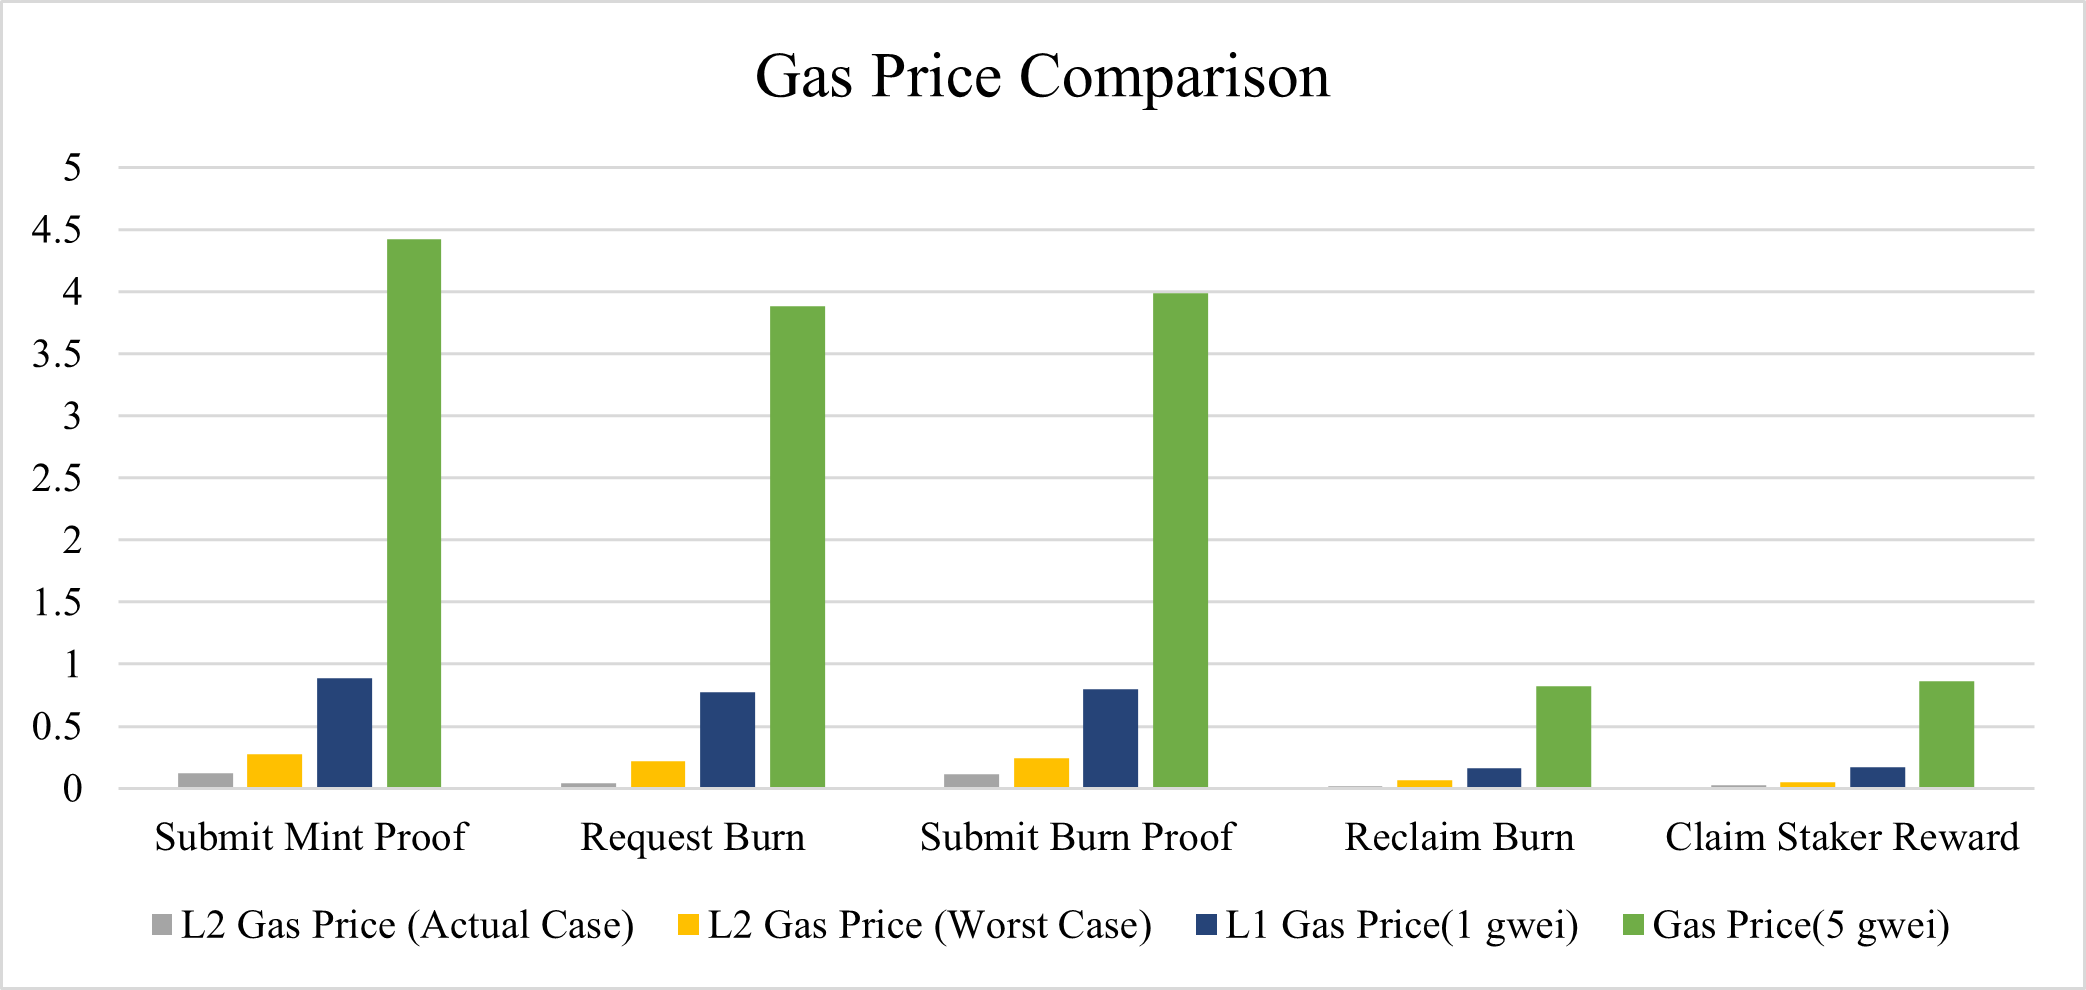
\includegraphics[width=1\textwidth]{img/gas_fee_comparison_2.png}
    \caption{Gas Price Comparison of Layer 1 (at 1 Gwei and 5 Gwei) and Layer 2 Deployment. Note: The 20 Gwei Layer 1 scenario is excluded to maintain visual clarity for other values.}
    \label{fig:gas_comparison}
\end{figure}


\subsection{Unit Testing}
Unit testing is a fundamental practice in smart contract development, crucial for ensuring the correctness, security, and reliability of the codebase. This section details the unit testing strategy employed for the \texttt{\zktoken} token smart contract, outlining the scope of tests and the specific functional areas covered.

\subsubsection{Testing Framework and Methodology}
The unit tests for the \texttt{\zktoken} token contract were developed using Foundry. This framework allowed for isolated testing of individual contract functions and their interactions, simulating various scenarios including valid inputs, edge cases, and expected error conditions. Each test case was designed to assert specific outcomes, such as successful state changes, correct value calculations, or appropriate transaction reverts. A total of 26 distinct test cases were implemented to achieve comprehensive coverage across the contract's functionalities.

\subsubsection{Functional Coverage}
The unit tests were systematically categorized and executed to cover all major functional areas of the \texttt{\zktoken} token contract, as outlined in its design. The primary functional areas and their corresponding test cases are detailed below:

\paragraph{Minting Logic (\texttt{verifyAndMint})}
This set of tests validates the integrity and correctness of the \texttt{verifyAndMint} function, which handles the issuance of \texttt{\zktoken} upon Bitcoin deposits.
\begin{itemize}
    \item \texttt{testVerifyAndMintHappyPath}: Verifies successful minting with valid inputs and correct fee distribution.
    \item \texttt{testVerifyAndMintMinAmount}: Confirms minting for the minimum allowable deposit amount.
    \item \texttt{testVerifyAndMintBelowMinAmount}: Asserts that transactions below the minimum minting amount correctly revert.
    \item \texttt{testVerifyAndMintInvalidProof}: Ensures the function reverts when an invalid ZK-proof is submitted.
    \item \texttt{testVerifyAndMintReuseTxId}: Validates that attempts to process a duplicate Bitcoin transaction ID (TXID) are correctly rejected to prevent double-minting.
\end{itemize}

\paragraph{Burning Logic (\texttt{initiateBurn}, \texttt{submitBurnProof}, \texttt{reclaimBurn})}
These tests assess the robustness of the burning process, including user-initiated requests, operator fulfillment, and the auto-recovery mechanism.
\begin{itemize}
    \item \texttt{testInitiateBurnHappyPath}: Verifies successful initiation of a burn request with valid parameters.
    \item \texttt{testInitiateBurnInsufficientBalance}: Asserts that burn requests with insufficient user balance correctly revert.
    \item \texttt{testInitiateBurnInvalidAmount}: Ensures the function reverts for burn amounts below the minimum threshold.
    \item \texttt{testSubmitBurnProofHappyPath}: Validates successful submission of a burn proof by an operator and subsequent \texttt{\zktoken} distribution.
    \item \texttt{testSubmitBurnProofAfterSubmissionPeriod}: Confirms that burn proof submissions after the designated challenge period correctly revert.
    \item \texttt{testReclaimBurnHappyPath}: Verifies successful reclamation of \texttt{\zktoken} by the user when an operator fails to submit a proof within the challenge period.
    \item \texttt{testReclaimBurnAlreadyClaimed}: Asserts that attempts to reclaim an already fulfilled or reclaimed burn request correctly revert.
    \item \texttt{testReclaimOpenRequest}: Ensures that users cannot reclaim funds for an open request before the challenge period expires.
\end{itemize}

\paragraph{Staker Initial Mint and Unlocking}
This category of tests verifies the mechanisms related to staker onboarding and the gradual release of their locked collateral.
\begin{itemize}
    \item \texttt{testStakerInitialMintOnDeploy}: Confirms that stakers receive their initial \texttt{\zktoken} mint upon contract deployment as specified.
    \item \texttt{testUnlockStakerTokensLinearUnlock}: Validates the correct linear unlocking of staker tokens over time.
    \item \texttt{testUnlockStakerTokensAfterFullPeriod}: Asserts that all unlockable tokens are available after the full unlocking period has elapsed.
    \item \texttt{testUnlockStakerTokensNothingToUnlock}: Ensures the function correctly handles scenarios where no tokens are available for unlocking.
    \item \texttt{testUnlockStakerTokensForeverLockedRemains}: Confirms that the designated `stakerForeverLocked` portion of collateral remains permanently locked.
    \item \texttt{testUnlockStakerTokensNonStakerReverts}: Asserts that non-staker addresses cannot invoke the unlock function.
    \item \texttt{testUnlockStakerTokensMultipleCalls}: Verifies that multiple calls to the unlock function are idempotent, correctly updating the unlocked amount without over-unlocking.
    \item \texttt{testStakerCannotTransferLockedTokens}: Ensures that stakers are prevented from transferring \texttt{\zktoken} that is still designated as locked collateral.
\end{itemize}

\paragraph{Staker Rewards (\texttt{claimStakerReward}, \texttt{distributeDust})}
These tests validate the integrity of the staker reward accumulation and claiming mechanisms.
\begin{itemize}
    \item \texttt{testClaimStakerReward}: Verifies successful claiming of accumulated staker rewards.
    \item \texttt{testClaimStakerRewardNoReward}: Asserts that attempts to claim rewards when none are available correctly revert.
    \item \texttt{testDistributeDust}: Confirms the correct distribution of accumulated dust amounts to the staker reward pool.
    \item \texttt{testDistributeDustTooLow}: Ensures the `distributeDust` function reverts if the accumulated dust is below the minimum threshold for distribution.
\end{itemize}

\paragraph{Admin Functions}
Tests in this category verify the proper functioning and access control of administrative functionalities.
\begin{itemize}
    \item \texttt{testChangeVerifierAddress}: Validates that the verifier contract address can be correctly updated by authorized parties.
    \item \texttt{testChangeProgramKeyMint/Burn}: Confirms that the ZK-proof program verification keys for both minting and burning circuits can be updated.
\end{itemize}

\subsubsection{Test Coverage Summary}
The comprehensive suite of 26 unit tests provides high functional coverage across all critical components of the \texttt{\zktoken} token smart contract. This rigorous testing approach contributes significantly to the confidence in the contract's correctness and adherence to its specified protocol logic, including its security mechanisms and economic model.


\section{Zero-Knowledge Proof System}
This section details the evaluation of the ZK-Proof generation process, focusing on generation time and proof size. The ZK-proofs were generated on a system with the following specifications: CPU Intel i5-13600k, 32GB RAM, and no NVIDIA GPU. Execution timestamps were logged during the ZK-Proof generation process. For robust analysis, each generation was performed five times, and the average values were utilized.

\begin{table}[h!]
\caption{ZK-Proof Generation Performance Metrics}
\label{tab:zkproof_performance}
\centering
\begin{tabular}{|l|c|c|l|}
\hline
\textbf{Phase} & \textbf{Mint Circuit} & \textbf{Burn Circuit} & \textbf{Notes} \\
\hline
generate main traces & 139 ms & 123 ms & Fast initial trace gen \\
prove\_core (overall) & 15.4 s & 15.0 s & Main proving workload \\
compress & 54.0 s & 52.7 s & Trace compression \\
shrink:prove\_shards & 7.54 s & 7.42 s & First phase of shrinking \\
shrink & 9.17 s & 9.03 s & Shrinking finalization \\
wrap\_bn254:prove\_shards & 67.9 s & 67.1 s & Groth16 wrapping shards \\
wrap\_bn254:verify & 111 ms & 110 ms & Verifying the wrapped shards \\
wrap\_bn254 (overall) & 96.0 s & 94.8 s & Final wrap \\
wrap\_groth16\_bn254:prove & 97.8 s & 24.2 s & Full Groth16 prover (docker) \\
\hline
\textbf{Total} & \textbf{298.35 s} & \textbf{270.48 s} & \\
\hline
\end{tabular}
\end{table}
As presented in Table~\ref{tab:zkproof_performance}, the total ZK-proof generation time for the minting circuit was 298.35 seconds, and for the burning circuit, it was 270.48 seconds. These results demonstrate the practical feasibility of generating complex ZK-proofs for Bitcoin state inclusion within reasonable timeframes, validating the computational viability of the bridge protocol. Furthermore, the generated proofs for both circuits are compact, with a size of 288 bytes each. This compact size is crucial for efficient on-chain verification, minimizing gas costs.
It is important to note that the SP1 zkVM supports NVIDIA GPU acceleration. Utilizing superior hardware configurations, including more powerful CPUs and increased RAM, or dedicated GPU resources, is expected to significantly reduce these generation times further.


\chapter{Discussion} \label{chap:discussion}
This chapter provides a comprehensive discussion of the proposed cross-chain bridge protocol. It begins by interpreting the key performance metrics obtained from the evaluation and conducts a comparative analysis against existing bridge solutions. Subsequently, the current limitations of the proof-of-concept are addressed, followed by an outline of future research and development opportunities.

\section{Determination of Protocol Fee Rates} \label{sec:fee_rate_determination}
As established in Section \ref{subsec:fee_determination}, the protocol fee rates for minting and burning, denoted by \(z\) and \(v\) respectively, are critically determined by the need to incentivize operators. These rates ensure that the operator's reward consistently exceeds their associated operational costs. For the current Proof-of-Concept (PoC) implementation, these fee rates are set as constants. However, in a fully functional version, they are envisioned to be dynamically adjustable parameters (a concept to be further explored in the Future Work section). This adjustability would allow the bridge to maintain operator incentivization during minor economic fluctuations, as gathering staker consensus for fee rate modifications may incur a time delay. Therefore, the chosen constant fee rates incorporate a buffer to absorb such fluctuations.

\subsubsection{Minting Fee Determination}
Recall the incentivization condition for the minting process, as derived in Equation 4.5:
\[
\alpha_{\text{BTC/USD}} \cdot \frac{X \cdot z}{2} > \alpha_{\text{ETH/USD}} \cdot C_{\text{Ethereum, mint}}
\]
Where \(X\) is the total amount of BTC the user intends to mint, \(z\) is the minting protocol fee rate, \(\alpha_{\text{BTC/USD}}\) is the Bitcoin to USD conversion ratio, \(\alpha_{\text{ETH/USD}}\) is the Ether to USD conversion ratio, and \(C_{\text{Ethereum, mint}}\) is the Ethereum gas cost for submitting the minting ZK-proof.

To evaluate the effectiveness of the chosen minting fee rate (0.1\% for this analysis), we analyze the inequality across various market conditions for BTC/USD and ETH/USD, alongside empirical gas cost data.

\paragraph{Assumed Market and Gas Parameters:}
\begin{itemize}
    \item \textbf{BTC/USD Conversion Ratios:} We consider a range of BTC prices at \$50,000, \$100,000, and \$150,000.
    \item \textbf{ETH/USD Conversion Ratios:} We consider a range of ETH prices at \$1,000, \$2,000, and \$4,000.
    \item \textbf{ZkSync Era Gas Price:} Based on a one-year historical record (July 4, 2024 - July 4, 2025) from the ZkSync block scout statistics \cite{noauthor_zksync_nodate}, the average gas price for the ZkSync Era network is consistently low and stable at approximately 0.044963 Gwei. This average is used for our calculations.
    \item \textbf{Gas Used for Minting ZK-Proof Submission:} From the evaluation in Section \ref{chap:evaluation} (specifically Table \ref{tab:l2_gas_metrics} in the "ZkSync Era Layer 2 Operational Costs" subsection), the \texttt{gasUsed} for the "Submit Mint Proof" operation on ZkSync Era Layer 2 is \textbf{1,073,014 gas units}  .
    \item \textbf{Minimum Minting Amount (\(X\)):} To maintain competitiveness with existing bridges, the minimum minting amount is set at \textbf{0.005 BTC}.
    \item \textbf{Minting Protocol Fee Rate (\(z\)):} For this analysis, the minting fee rate is set at \textbf{0.1\% (0.001)} of the transacted amount.
\end{itemize}

\paragraph{Calculation of Operator's Operational Cost (Right-Hand Side of Inequality):}
The operator's Ethereum operational cost, denoted as 
\(\alpha_{\text{ETH/USD}} \cdot C_{\text{Ethereum, mint}}\), 
is calculated using the following expression:

\[
\text{GasUsed} \times \text{GasPrice}_{\text{avg}} \times 10^{-9} \times \alpha_{\text{ETH/USD}}
\]

where:
\begin{itemize}
    \item \(\text{GasUsed} = 1,\!073,\!014\) is the gas consumed on zkSync,
    \item \(\text{GasPrice}_{\text{avg}} = 0.044963\) Gwei is the average gas price,
    \item \(10^{-9}\) converts Gwei to ETH,
    \item \(\alpha_{\text{ETH/USD}}\) is the ETH-to-USD conversion rate.
\end{itemize}

\begin{align*}
C_{\text{Ethereum, mint (USD)}} &= 1,073,014 \times 0.044963 \times 10^{-9} \times \alpha_{\text{ETH/USD}} \\
&= 0.000048246 \times \alpha_{\text{ETH/USD}}
\end{align*}

The estimated operational costs under varying ETH/USD rates are presented in Table \ref{tab:minting_cost_rhs}.

\begin{table}[h!]
\caption{Estimated Operator Minting Operational Costs (USD)}
\label{tab:minting_cost_rhs}
\centering
\begin{tabular}{|l|c|c|c|}
\hline
\textbf{ETH/USD} & \textbf{\$1,000} & \textbf{\$2,000} & \textbf{\$4,000} \\
\hline
Cost (\(\alpha_{\text{ETH/USD}} \cdot C_{\text{Ethereum, mint}}\)) & \$0.048246 & \$0.096492 & \$0.192984 \\
\hline
\end{tabular}
\end{table}

\paragraph{Calculation of Operator's Reward (Left Hand Side of Inequality):}
The operator's reward (\(\alpha_{\text{BTC/USD}} \cdot \frac{X \cdot z}{2}\)) is calculated using the minimum minting amount (\(X = 0.005\) BTC) and the chosen fee rate (\(z = 0.001\)):

\begin{align*}
R_{\text{operator, mint (USD)}} &= \alpha_{\text{BTC/USD}} \cdot \frac{0.005 \cdot 0.001}{2} \\
&= \alpha_{\text{BTC/USD}} \cdot \frac{0.000005}{2} \\
&= \alpha_{\text{BTC/USD}} \cdot 0.0000025
\end{align*}

The estimated operator rewards under varying BTC/USD rates are presented in Table \ref{tab:minting_reward_lhs}.

\begin{table}[h!]
\caption{Estimated Operator Minting Rewards (USD)}
\label{tab:minting_reward_lhs}
\centering
\begin{tabular}{|l|c|c|c|}
\hline
\textbf{BTC/USD} & \textbf{\$50,000} & \textbf{\$100,000} & \textbf{\$150,000} \\
\hline
Reward (\(\alpha_{\text{BTC/USD}} \cdot R_{\text{operator, mint}}\)) & \$0.125 & \$0.250 & \$0.375 \\
\hline
\end{tabular}
\end{table}

\paragraph{Analysis of Incentivization Condition for Minting:}
Comparing the values from Table \ref{tab:minting_reward_lhs} (operator reward) with Table \ref{tab:minting_cost_rhs} (operator operational cost), we observe that the operator's reward consistently surpasses their operational cost under most analyzed market scenarios. This indicates that a 0.1\% minting fee rate (for a 0.005 BTC minimum minting amount) generally provides sufficient incentive.

However, a specific edge case arises when BTC/USD is at its lowest analyzed point (\$50,000) and ETH/USD is at its highest (\$4,000). In this scenario, the operator's reward (\$0.125) falls below the operational cost (\$0.192984), meaning the incentivization condition is not met. It is important to note that BTC/USD and ETH/USD typically exhibit a high correlation, making such extreme divergence less likely to occur. Should such a scenario materialize, stakers would need to adjust either the minimum minting amount or the protocol fee rate to re-establish operator profitability.

This analysis confirms that the chosen 0.1\% minting fee rate offers a robust incentive for operators across a wide range of typical market conditions, with a defined edge case that highlights the need for a dynamic fee adjustment mechanism in a production environment.

\subsubsection{Burning Fee Determination}
Similarly, the fee rate for the burning process (\(v\)) is determined by ensuring the operator's reward surpasses their operational costs. As recalled from Equation 4.6 in Section \ref{subsec:fee_determination}:
\[
\alpha_{\text{BTC/USD}} \cdot \frac{Y \cdot v}{2} > \alpha_{\text{BTC/USD}} \cdot C_{\text{Bitcoin}} + \alpha_{\text{ETH/USD}} \cdot C_{\text{Ethereum, burn}}
\]
Where \(Y\) is the total amount of \texttt{\zktoken} the user intends to burn, \(v\) is the burning protocol fee rate, \(\alpha_{\text{BTC/USD}}\) and \(\alpha_{\text{ETH/USD}}\) are the respective conversion ratios to USD. \(C_{\text{Bitcoin}}\) represents the Bitcoin transaction fee for fronting BTC, and \(C_{\text{Ethereum, burn}}\) is the Ethereum gas cost for submitting the burning ZK-proof.

A key distinction from the minting process is that the operator's cost in the burning process encompasses two components: the gas fee for submitting the ZK-proof to Ethereum Layer 2, and the transaction fee for sending BTC to the user on the Bitcoin network. Therefore, a comprehensive estimation of both these costs is crucial.

\paragraph{Assumed Market and Gas Parameters:}
The same market conversion ratio ranges for BTC/USD and ETH/USD are used as in the minting fee determination:
\begin{itemize}
    \item \textbf{BTC/USD Conversion Ratios:} \$50,000, \$100,000, and \$150,000.
    \item \textbf{ETH/USD Conversion Ratios:} \$1,000, \$2,000, and \$4,000.
    \item \textbf{ZkSync Era Gas Price:} The average gas price of 0.044963 Gwei is maintained.
    \item \textbf{Gas Used for Burning ZK-Proof Submission:} From the evaluation in Section \ref{chap:evaluation} (specifically Table \ref{tab:l2_gas_metrics}), the \texttt{gasUsed} for the "Submit Burn Proof" operation on ZkSync Era Layer 2 is \textbf{1,046,366 gas units}.
    \item \textbf{Minimum Burning Amount (\(Y\)):} The minimum burning amount is set at \textbf{0.01 BTC}.
    \item \textbf{Burning Protocol Fee Rate (\(v\)):} For this analysis, the burning fee rate is set at \textbf{0.15\% (0.0015)} of the transacted amount.
\end{itemize}

\paragraph{Estimation of Operator's Operational Costs (Right-Hand Side of Inequality)}

\subparagraph{Ethereum Operational Cost (\(\alpha_{\text{ETH/USD}} \cdot C_{\text{Ethereum, burn}}\)):}
The operator’s cost to submit the burn proof on Ethereum is calculated using the following formula:

\[
C_{\text{Ethereum, burn (USD)}} = G \times P \times 10^{-9} \times \alpha_{\text{ETH/USD}}
\]

where:
\begin{itemize}
    \item \(G = 1,\!046,\!366\) is the gas used on zkSync for the burn proof,
    \item \(P = 0.044963\) Gwei is the average gas price,
    \item \(10^{-9}\) converts Gwei to ETH,
    \item \(\alpha_{\text{ETH/USD}}\) is the ETH-to-USD conversion rate.
\end{itemize}

Substituting the values:

\begin{align*}
C_{\text{Ethereum, burn (USD)}} &= 1,\!046,\!366 \times 0.044963 \times 10^{-9} \times \alpha_{\text{ETH/USD}} \\
&= 0.000047048 \times \alpha_{\text{ETH/USD}}
\end{align*}

The estimated Ethereum operational costs under varying ETH/USD exchange rates are summarized in Table~\ref{tab:burning_eth_cost}.


\begin{table}[h!]
\caption{Estimated Operator Burning Ethereum Costs (USD)}
\label{tab:burning_eth_cost}
\centering
\begin{tabular}{|l|c|c|c|}
\hline
\textbf{ETH/USD} & \textbf{\$1,000} & \textbf{\$2,000} & \textbf{\$4,000} \\
\hline
Cost (\(\alpha_{\text{ETH/USD}} \cdot C_{\text{Ethereum, burn}}\)) & \$0.047048 & \$0.094096 & \$0.188192 \\
\hline
\end{tabular}
\end{table}

\subparagraph{Bitcoin Transaction Cost (\(\alpha_{\text{BTC/USD}} \cdot C_{\text{Bitcoin}}\)):}
The Bitcoin transaction fee is estimated based on average network conditions. We consider the 25th percentile median fee rate over the past year for slow confirmation (~3.0394 sat/vB), which typically ensures inclusion within several hours, well within the predefined 1-day burn request window. \cite{noauthor_bitcoin_2025}

For a standard Bitcoin transaction, assuming a SegWit address with 1 input and 2 outputs, the transaction size can be estimated as 1 input \(\times\) 68.5 vbytes + 2 outputs \(\times\) 31 vbytes + 10 vbytes (base) \(= 140.5\) vbytes, rounded to \textbf{141 vbytes} \cite{noauthor_bitcoin_nodate}.

Total Fee (satoshis) = Transaction Size (vbytes) \(\times\) Fee Rate (satoshis/vbyte)
Total Fee = 141 vbytes \(\times\) 3.0394 sat/vB \(\approx\) 428.56 satoshis. For simplicity in calculation, we round to \textbf{429 satoshis}.

The estimated Bitcoin transaction costs under varying BTC/USD rates are presented in Table \ref{tab:burning_btc_cost}.

\begin{table}[h!]
\caption{Estimated Operator Burning Bitcoin Costs (USD)}
\label{tab:burning_btc_cost}
\centering
\begin{tabular}{|l|c|c|c|}
\hline
\textbf{BTC/USD} & \textbf{\$50,000} & \textbf{\$100,000} & \textbf{\$150,000} \\
\hline
Cost (\(\alpha_{\text{BTC/USD}} \cdot C_{\text{Bitcoin}}\)) & \$0.2145 & \$0.4290 & \$0.6435 \\
\hline
\end{tabular}
\end{table}

\subparagraph{Total Operational Cost (Right Hand Side of Inequality):}
The total operational cost for the operator is the sum of the Ethereum and Bitcoin costs. Table \ref{tab:total_burning_cost} presents these combined costs across various market scenarios.

\begin{table}[h!]
\caption{Total Estimated Operator Burning Operational Costs (USD)}
\label{tab:total_burning_cost}
\centering
\begin{tabular}{|c|c|c|c|}
\hline
\textbf{BTC/USD} \(\downarrow\) / \textbf{ETH/USD} \(\rightarrow\) & \textbf{\$1,000} & \textbf{\$2,000} & \textbf{\$4,000} \\
\hline
\textbf{\$50,000} &  \cellcolor{gray!20}\$0.258548 & \$0.305596 & \$0.399619 \\
\hline
\textbf{\$100,000} & \$0.470048 & \cellcolor{gray!20}\$0.517096 & \$0.611119 \\
\hline
\textbf{\$150,000} & \$0.681548 & \$0.728596 & \cellcolor{gray!20}\$0.822619 \\
\hline
\end{tabular}
\end{table}

\paragraph{Calculation of Operator's Reward (Left Hand Side of Inequality):}
The operator's reward (\(\alpha_{\text{BTC/USD}} \cdot \frac{Y \cdot v}{2}\)) is calculated using the minimum burning amount (\(Y = 0.01\) BTC) and the chosen fee rate (\(v = 0.0015\)):

\begin{align*}
R_{\text{operator, burn (USD)}} &= \alpha_{\text{BTC/USD}} \cdot \frac{0.01 \cdot 0.0015}{2} \\
&= \alpha_{\text{BTC/USD}} \cdot \frac{0.000015}{2} \\
&= \alpha_{\text{BTC/USD}} \cdot 0.0000075
\end{align*}

The estimated operator rewards under varying BTC/USD rates are presented in Table \ref{tab:burning_reward_lhs}.

\begin{table}[h!]
\caption{Estimated Operator Burning Rewards (USD)}
\label{tab:burning_reward_lhs}
\centering
\begin{tabular}{|l|c|c|c|}
\hline
\textbf{BTC/USD} & \textbf{\$50,000} & \textbf{\$100,000} & \textbf{\$150,000} \\
\hline
Reward (\(\alpha_{\text{BTC/USD}} \cdot R_{\text{operator, burn}}\)) & \$0.375 & \$0.750 & \$1.125 \\
\hline
\end{tabular}
\end{table}

\paragraph{Analysis of Incentivization Condition for Burning:}
Comparing the operator's reward (Table \ref{tab:burning_reward_lhs}) with the total operational cost (Table \ref{tab:total_burning_cost}), we observe that the operator's reward consistently exceeds their combined operational costs across all analyzed market scenarios. This robust margin ensures that a 0.15\% burning fee rate, in conjunction with a 0.01 BTC minimum burn amount, provides sufficient and consistent incentive for operators, even under the most unfavorable assumed market conditions (e.g., high ETH/USD, low BTC/USD). This demonstrates the economic viability of the burning process within the proposed model.

\subsection{Comparison with Existing Trust-Minimized Bridges} \label{subsec:performance_comparison}
This section provides a comparative analysis of our proposed \texttt{\zktoken} bridge against \texttt{tBTC v2}, a notable decentralized cross-chain bridge, across key criteria: security model, minimum deposit amounts, protocol fee rates, and transaction times.

\paragraph{Trust Model}
\texttt{tBTC v2} operates on a Threshold ECDSA signing mechanism, bolstered by slashing penalties and watchtowers to maintain integrity and responsiveness. Its security fundamentally relies on the honesty of a majority of its signers, with economic incentives and cryptographic assurances guiding their behavior toward system security.

In contrast, our \texttt{\zktoken} bridge significantly enhances trust minimization. All operations critical to maintaining the peg, such as minting and burning, are secured by Zero-Knowledge Proofs, eliminating the need for external relays or oracles for transaction inclusion verification. Furthermore, the bridge's underlying Bitcoin fund is managed using a Threshold Schnorr Signature (TSS) scheme (specifically Frost Sign, which generates Schnorr signatures). This TSS implementation is designed to be secure as long as at least one participant remains honest. This design principle positions \texttt{\zktoken} to offer a higher degree of trust minimization compared to majority-based multisignature schemes.

\paragraph{Minimum Deposit and Fee Rates}
The accessibility and cost-effectiveness of a bridge are significantly influenced by its minimum deposit requirements and fee structures. A direct comparison of these metrics for \texttt{tBTC v2} and \texttt{\zktoken} is presented in Table \ref{tab:bridge_comparison}.

\begin{table}[h!]
\centering
\begin{tabularx}{\textwidth}{|X|X|X|X|}
\hline
\textbf{Feature / Metric} & \textbf{tBTC v2} & \textbf{\zktoken} & \textbf{Notes / Differentiator} \\
\hline
\textbf{Trust Model} & Threshold multi-signature (Majority) & ZK-proofs + TSS (Cryptographic + 1 honest participant) & More granular trust minimization \\
\hline
\textbf{Minimum Deposit} & 0.01 BTC & 0.0001 BTC & Enhances accessibility \\
\hline
\textbf{Mint Fee} & 0\% & 0.2\% & Efficient operator incentives \\
\hline
\textbf{Burn Fee} & 0.2\% & 0.2\% & Efficient operator incentives \\
\hline
\textbf{Mint Time} & \(\sim\) 1--3 hrs & \(\sim\) 1 hr & Faster Confirmation \\
\hline
\textbf{Burn Time} & \(\sim\) 3--5 hrs & \(\sim\) 1 hr & Faster Confirmation \\
\hline
\end{tabularx}
\caption{Comparison between tBTC v2 and \zktoken}
\label{tab:bridge_comparison}
\end{table}

\texttt{\zktoken} significantly lowers the liquidity barrier for users, with a minimum deposit amount of 0.0001 BTC, which is 100 times smaller than \texttt{tBTC v2}'s 0.01 BTC. This substantially enhances accessibility for users with smaller asset holdings. Regarding fee rates, \texttt{tBTC v2} offers a 0\% minting fee, whereas \texttt{\zktoken} implements a 0.2\% minting fee. Both bridges maintain a 0.2\% burn fee. While \texttt{\zktoken}'s individual minting fee is higher, its design prioritizes efficient operator incentives, which is crucial for the long-term sustainability and liquidity of the bridge. Future work will explore refining the economic model to potentially optimize these fee rates while maintaining robust incentivization and considering the overall combined fee for both operations.

\paragraph{Transaction Times}
Transaction finality is a critical user experience factor. \texttt{tBTC v2} typically processes minting operations within 1 to 3 hours, and burning operations take between 3 to 5 hours. Our \texttt{\zktoken} bridge, on the other hand, offers significantly faster transaction times. Both minting and burning operations are primarily dependent on achieving 6 Bitcoin transaction confirmations, which ideally takes approximately 1 hour. This consistent and faster confirmation time provides a notable advantage for \texttt{\zktoken} users seeking quicker cross-chain transfers.

\paragraph{Summary}
In conclusion, while \texttt{\zktoken} currently presents a higher minting fee compared to \texttt{tBTC v2}, it distinguishes itself through a more granular trust minimization model, significantly enhanced accessibility via a lower minimum deposit, and notably faster minting and burning times. These attributes position \texttt{\zktoken} as a robust, faster, and more secure alternative in the trust-minimized cross-chain bridge landscape.


\section{Limitations} \label{sec:limitations}
This section outlines the current limitations observed in the developed Proof-of-Concept (PoC) cross-chain bridge protocol. Addressing these limitations represents key areas for future research and development.

\subsection{Kickstart Phase Centralization} \label{subsec:kickstart_limitation}
In the current PoC, the initial kickstart phase, which encompasses the Distributed Key Generation (DKG) for the Threshold Signature Scheme (TSS) setup and the subsequent smart contract deployment, is centrally managed by the development team. This centralized control ensures a smooth and guaranteed operation for demonstration purposes. However, a fully decentralized deployment necessitates an "all-or-nothing" atomic commitment mechanism. This mechanism would ensure that either all initial stakers successfully fund their commitments and the smart contract becomes operational, or no funds (or associated gas fees) are expended by any participant. The design and implementation of such a truly decentralized kickstart process, ensuring this atomicity without central coordination, remain a significant area for future work.


\subsection{Proof-of-Fulfillment Race Condition and Operator Disincentive}

A significant limitation in the current protocol design is a potential race condition in the burn fulfillment process. The protocol separates the action of fulfilling a burn request (an operator fronting their own BTC to a user) from the action of claiming the reward (submitting a ZK-proof of the fulfillment transaction to the smart contract). Because the fulfillment transaction is public on the Bitcoin blockchain, any observer can construct a ZK-proof for it.

This creates an attack vector where a malicious or opportunistic operator (Operator B) can "snipe" the proof submission. The scenario unfolds as follows:
\begin{enumerate}
    \item An honest operator (Operator A) fronts their BTC to fulfill a user's burn request.
    \item Operator B monitors the blockchain, sees Operator A's transaction, and immediately begins generating their own ZK-proof for that same transaction.
    \item A race ensues to submit the proof to the token smart contract. If Operator B is faster, they will receive the reimbursement and reward intended for Operator A.
\end{enumerate}

In this case, Operator A suffers a direct financial loss of the fronted BTC and wastes the computational resources used for proof generation. This vulnerability creates a strong economic disincentive for any operator to be the first to fulfill a burn request. It encourages a "wait-and-see" behavior, where operators may hesitate to front funds, instead preferring to race to prove a fulfillment transaction initiated by someone else. This could severely degrade the liveness and reliability of the bridge's burn mechanism.

\subsection{Operator Liquidity and Staker Consensus Risk} \label{subsec:liquidity_limitation}
As discussed in Section \ref{sec:trust-model-and-assumption}, the protocol relies on two key assumptions related to operator liquidity and staker behavior. Firstly, it assumes that operators will consistently possess sufficient liquidity to fulfill burn requests. Secondly, it assumes that stakers are rational and will unanimously cooperate to release liquidity from the bridge's locked funds in scenarios where operators' individual liquidity is insufficient. These two assumptions are interdependent and are posited to collectively ensure the bridge's continuous functionality.

However, in a real-world scenario, the practical availability of operator-fronted BTC liquidity might fluctuate, and there is an inherent risk that stakers may not always achieve unanimous consensus for liquidity release, particularly during stressed market conditions or disputes. Should these assumptions fail to hold—specifically, if operators lack the necessary liquidity for burn requests and stakers cannot reach an immediate, unanimous agreement for liquidity provision—the bridge could effectively become a "one-way" bridge. In such an event, the minting process would remain functional, allowing new \texttt{\zktoken} to be issued, but the corresponding locked BTC on the Bitcoin network would become irretrievable, preventing users from burning their \texttt{\zktoken} back to native BTC.

\subsection{Threshold Signature Incompatibility} \label{subsec:tss_incompatibility}
The current PoC utilizes Threshold Schnorr Signatures for managing the Bitcoin-side funds. While Schnorr signatures are natively supported and highly efficient on the Bitcoin network, they are not directly compatible with the Ethereum Virtual Machine (EVM). This incompatibility necessitates that for a full and seamless integration with the Ethereum ecosystem, future iterations of the bridge would need to adopt a TSS protocol that supports ECDSA signatures, which are natively compatible with Ethereum.

\subsection{Hard-Coded Constants} \label{subsec:hardcoded_constants}
A current limitation of the PoC lies in the presence of hard-coded constants within both the Zero-Knowledge (ZK) circuit implementation and the associated smart contracts. For enhanced flexibility and dynamism, future development should aim to externalize these constants. This would involve designing the ZK circuit to accept such constants as variables, which would then be included as public inputs during ZK-Proof generation. Similarly, constants within the token smart contract could be made configurable by stakers through governance mechanisms, allowing for dynamic adjustments to protocol parameters.

It is crucial to acknowledge, however, that increasing the number of public outputs in a ZK circuit directly correlates with higher computational and gas costs for ZK-Proof submission on the Ethereum Layer 2. Therefore, a meticulous design approach will be indispensable to carefully balance the benefits of dynamic flexibility and decentralized control against the associated operational expenses to ensure the bridge remains economically viable and efficient.

\section{Future Work}
Building upon the insights gained from the evaluation and acknowledging the identified limitations, this section outlines potential avenues for future research and development aimed at enhancing the robustness, decentralization, and practicality of the \texttt{\zktoken} bridge.

\subsection{Developing a Trust-Minimized Kickstart Protocol} \label{subsec:trust_minimized_kickstart}
As highlighted in the limitations, the PoC relies on a centralized kickstart phase. Future work must focus on designing and implementing a decentralized, "all-or-nothing" atomic setup protocol to ensure that either all stakers successfully fund their commitments and deploy the bridge, or no assets are spent.

The proposed solution involves a coordinated, two-phase process. First, the designated stakers would use a \textbf{Threshold-ECDSA Distributed Key Generation (DKG)} protocol. This is critical because a single ECDSA key pair can deterministically control both a Bitcoin address (e.g., P2WPKH) and an Ethereum address, creating a unified cryptographic identity across both chains.

Second, the stakers would collaboratively construct and partially sign two parallel transaction packets: a \textbf{Partially Signed Bitcoin Transaction (PSBT)} committing their individual UTXOs to the new bridge address, and a signed \textbf{Ethereum contract creation transaction}. A strict "atomic release rule" based on social consensus would ensure that neither transaction is broadcast until both are fully signed by all stakers. This provides censorship resistance, as any staker can broadcast the final transactions, and prevents premature execution. For enhanced auditability, a hash of the Ethereum transaction could be embedded in the Bitcoin transaction via an \texttt{OP\_RETURN} output, creating a cryptographic link.

To move beyond social consensus and achieve true cryptographic atomicity, this protocol could be further enhanced with advanced techniques. For instance, \textbf{Hash Time Locked Contracts (HTLCs)} could be used to make the funding of the Bitcoin transaction dependent on revealing a secret that is also required for the Ethereum contract's successful deployment. Alternatively, \textbf{Adaptor Signatures} could ensure that the final signature for the Bitcoin transaction simultaneously reveals the necessary data to complete the Ethereum transaction signature, creating a direct cryptographic dependency.

Implementing this trust-minimized kickstart phase would involve overcoming several engineering challenges, including the pre-funding of gas for the Ethereum deployment and managing nonce sequencing for future upgrades. However, this approach provides a clear path toward a fully decentralized and robust deployment mechanism, a crucial step in moving the protocol from a PoC to a production-ready system.

\subsection{Enhancing Burn Fulfillment with Proof of Ownership}

To mitigate the proof-sniping vulnerability identified in the limitations, future work must focus on cryptographically linking the ZK-proof of fulfillment to the operator who genuinely sent the funds. This can be achieved by enhancing the ZK-circuit for the burn process to not only prove transaction inclusion but also to verify the operator's ownership of the transaction's inputs.

The proposed solution involves modifying the circuit to accept the operator's private key(s) as a private witness. Inside the circuit, the following assertions would be enforced for each input UTXO in the fulfillment transaction:
\begin{enumerate}
    \item \textbf{Public Key Derivation:} The circuit would take the operator's private key (witness) and use elliptic curve multiplication to re-derive the corresponding public key.
    \item \textbf{Signature Regeneration:} The circuit would use the private key witness and the transaction data to re-create the ECDSA signature for that input.
    \item \textbf{Consistency Assertion:} The circuit would then assert that the re-derived public key matches the public key of the original input and that the re-created signature matches the original signature on the transaction.
\end{enumerate}

By enforcing these checks, the circuit guarantees that \textbf{only the true owner of the input UTXOs—the operator who actually fronted the BTC—can generate a valid proof}. This eliminates the race condition entirely.

This design must also account for transactions with multiple inputs, which would require the operator to provide multiple private key witnesses. The core logic remains the same: the circuit must prove ownership over \textit{every} input UTXO consumed in the fulfillment transaction. Implementing this "proof of ownership" would remove the fear of fronting funds and significantly enhance the robustness and fairness of the protocol's burn mechanism.



\subsection{Change of Threshold Algorithm} \label{subsec:future_tss_change}
As previously discussed in Section \ref{subsec:tss_incompatibility}, the current Proof-of-Concept (PoC) implementation of the \texttt{\zktoken} bridge utilizes Threshold Schnorr Signatures. While Schnorr signatures offer advantages such as native support on the Bitcoin network and enable Taproot compatibility, they are not natively supported by the Ethereum Virtual Machine (EVM). This incompatibility necessitates a distinct signature mechanism for Ethereum-side operations if a single, unified key derivation process is not employed.

For a more streamlined and robust system in a production environment, future work will focus on transitioning to a Threshold ECDSA Signature scheme. ECDSA is natively supported by both Bitcoin (for P2PKH and P2WPKH addresses) and Ethereum (for EOAs). By adopting Threshold ECDSA, stakers could derive and control both their Bitcoin and Ethereum accounts using a unified set of cryptographic shares. This approach significantly reduces the overall system complexity by eliminating the need for two separate signing algorithms or cumbersome cross-chain key derivations, thereby enhancing the holistic security posture and simplifying operational overhead for stakers.

\subsection{Refinement of Fee Rates and Minimum Transaction Amounts} \label{subsec:future_fee_refinement}
As demonstrated in Section \ref{sec:fee_rate_determination}, the current fixed fee rates and minimum mint/burn amounts for the PoC were determined through an analysis designed to ensure operator incentivization and bridge functionality across a wide range of Bitcoin and Ethereum market fluctuations. This determination considered factors such as the economic endurability for operators, maintaining competitiveness, and accommodating for potential delays in staker consensus for parameter adjustments.

While the current PoC bridge may not outperform competitors like \texttt{tBTC v2} solely in terms of fee rates, it offers significant advantages in its trust model, security, and operational speed. Therefore, a crucial area for future development involves exploring and implementing dynamic adjustment mechanisms for protocol fee rates and minimum transaction amounts. With the establishment of a robust and responsive staker community capable of timely voting and parameter modifications, it may be feasible to refine the fee structure further. This could potentially lead to a reduction in the overall fee burden, enabling \texttt{\zktoken} to match or even surpass the competitiveness of existing solutions, particularly when its inherent security and efficiency advantages are considered. This future work would involve careful economic modeling and community governance design to optimize the balance between operator incentives, user costs, and system resilience.

\chapter{Conclusion} \label{chap:conclusion}
\thispagestyle{empty}

This thesis began by identifying a critical challenge at the intersection of blockchain's most prominent networks: Bitcoin's constrained scalability and the security vulnerabilities inherent in cross-chain bridges designed to connect it to Ethereum's powerful Layer 2 ecosystem. The research established a clear need for a new generation of interoperability solutions that could move beyond centralized or federated trust models. In response, this work set out to design, implement, and evaluate a Proof-of-Concept (PoC) for a trust-minimized bridge, exploring a novel architecture to address this gap.

\section{Summary of Contributions}

This thesis addressed the problem of secure Bitcoin-to-Ethereum interoperability by delivering a tangible and empirically validated PoC. The core contribution is a novel, hybrid architecture for a trust-minimized bridge, whose components and design principles stand as a direct response to the limitations of existing systems.

The approach was threefold, integrating modern cryptographic primitives with a strategic L2 deployment:
\begin{enumerate}
    \item \textbf{Decentralized Custody} was achieved using a \textbf{Threshold Signature Scheme (TSS)}, specifically the FROST protocol, which secures Bitcoin funds without a single point of failure.
    \item \textbf{Verifiable State Transitions} were enforced using \textbf{Zero-Knowledge Proofs (ZKPs)}, allowing for the verification of Bitcoin transaction inclusion on an Ethereum L2 without relying on trusted external relays or oracles.
    \item \textbf{On-Chain Logic and Asset Representation} was managed by a custom \textbf{ERC-20 token smart contract}, deployed on the ZkSync Era rollup to ensure economic viability.
\end{enumerate}

The unique contribution of this work is not just in the individual components, but in their synthesis. By building and evaluating this system, this thesis delivers: a working PoC of a trust-minimized mint/burn mechanism; a protocol design that directly confronts the trade-offs of capital efficiency and security identified in state-of-the-art bridges like tBTC v2 and BitVM; and a set of empirical benchmarks that ground the theoretical design in practical performance metrics.

\section{Synthesis of Evaluation and Discussion}

The empirical results, when viewed holistically, validate the fundamental feasibility of the proposed architecture while simultaneously illuminating the practical trade-offs inherent in its design. This PoC moves beyond theoretical claims to provide a clear picture of what such a system entails in practice.

The evaluations collectively show that the core cryptographic operations are not prohibitive bottlenecks. The TSS component for decentralized custody completes in milliseconds in local network, while the compact size of the ZK-proofs (288 bytes) makes on-chain verification efficient. The most critical finding is the \textbf{economic viability granted by the Layer 2 deployment} , which reduces operational gas costs by 85-98\% compared to a L1 deployment, confirming that such advanced bridges are only practical on rollups.

However, the analysis also reveals a key architectural trade-off:\textbf{cryptographic security at the cost of guaranteed operational liveness} . The Discussion highlighted that the protocol's ultimate ability to process redemptions depends on a crucial socio-economic assumption: the consistent availability of operator liquidity, backed by staker consensus. A failure of this assumption presents the primary risk of the bridge becoming "one-way"—where minting continues but burning stalls—a limitation that underscores the challenge of designing fully robust decentralized systems. The project thus establishes a delicate balance: it achieves strong cryptographic trust-minimization for fund safety but makes its operational liveness contingent on explicit economic incentives and rational actor behavior.

\section{Broader Implications}

The findings of this thesis carry several broader implications for the future of blockchain interoperability and decentralized infrastructure.

First, the hybrid model presented here offers a valuable blueprint for future bridge designs. It suggests that a departure from monolithic security models (e.g., purely honest-majority or purely 1-of-n) towards modular systems that combine different cryptographic and economic primitives can yield a more balanced and practical set of trade-offs.

Second, for Bitcoin-Ethereum interoperability, this work reinforces that leveraging Ethereum's L2 ecosystem is the most viable path forward. It demonstrates that the programmability of L2s can be used to enforce complex verification logic—like ZKP verification—that would be impossible on Bitcoin's base layer, effectively outsourcing Bitcoin's scaling to a more flexible environment.

Finally, this research contributes to the practical understanding of trust-minimized systems. By providing empirical data on the real-world costs and latencies of advanced cryptographic protocols in a blockchain context, it moves the conversation from purely theoretical designs to benchmarked implementations, offering a more grounded perspective for developers and researchers.

\section{Final Remarks}

While the system developed in this thesis remains a Proof-of-Concept, its contribution is significant. It establishes the architectural groundwork for practical and secure Bitcoin-Ethereum interoperability that moves beyond the limitations of federated custody. This work validates that through a careful synthesis of modern cryptography and Layer 2 technology, the promise of unlocking Bitcoin's vast liquidity within a programmable, scalable ecosystem is not only possible, but is within practical reach.



%%%%%%%%%%%%%%%%%%%%% Bibliography %%%%%%%%%%%%%%%%%%%%%% 
\addcontentsline{toc}{chapter}{Bibliography}
\printbibliography
\end{document}  